% ==============================================================================
% sci_tutorial_core.tex — SCI/SICE tutorial 2026, "core" (要点版) deck.
% SCI/SICE チュートリアル講座 2026 スライド「要点版」。
%
% The full deck (sci_tutorial.tex) is kept as it is. This deck contains only
% what a participant does and needs to know, in the order the participant
% follows (6 steps), not in timetable order. No "read later" frames.
% 現行版 (sci_tutorial.tex) はそのまま残す。本デッキは受講者が「やること」と
% 「知る必要があること」だけを、時間割ではなく受講者がたどる順（6 ステップ）で
% 並べる。「あとで読む」フレームは入れない。
%
% Build / ビルド:  cd docs/events && make sci-core
% ==============================================================================
\documentclass[aspectratio=169, 14pt, t]{beamer}
\usepackage{stampfly_slides}
\input{preamble}
\usepackage{ccicons}   % Creative Commons icons for the title page / 表紙の CC アイコン

% --- License notice on the title page (same as the full deck) ---------------
% 表紙のライセンス表示（現行版と同じ）。
\newcommand{\sciLicenseIcon}{\ccby}
\newcommand{\sciLicenseText}{この資料は CC BY 4.0（クリエイティブ・コモンズ 表示 4.0 国際）で公開}
\newcommand{\sciLicenseURL}{https://creativecommons.org/licenses/by/4.0/deed.ja}

% --- Footer: current step | course title + lecturer | page ------------------
% Same override as the full deck (shared style file untouched).
% \sciFooterSession is updated by \scistep.
% 現行版と同じ方針でフッターを置き換える（共有スタイルは触らない）。
% \sciFooterSession は \scistep が更新する。
\newcommand{\sciFooterSession}{}
\newcommand{\sciFooterTitle}{制御教育教材 StampFly Ecosystem の紹介（要点版） ｜ 伊藤 恒平（金沢工業大学）}
\setbeamertemplate{footline}{%
  \leavevmode\hbox{%
    \begin{beamercolorbox}[wd=.26\paperwidth,ht=2.5ex,dp=1ex,center]{palette primary}%
      \usebeamerfont{author in head/foot}\sciFooterSession
    \end{beamercolorbox}%
    \begin{beamercolorbox}[wd=.59\paperwidth,ht=2.5ex,dp=1ex,center]{palette secondary}%
      \usebeamerfont{title in head/foot}\sciFooterTitle
    \end{beamercolorbox}%
    \begin{beamercolorbox}[wd=.15\paperwidth,ht=2.5ex,dp=1ex,right]{palette tertiary}%
      \usebeamerfont{date in head/foot}%
      \insertframenumber{} / \inserttotalframenumber\hspace*{2ex}
    \end{beamercolorbox}%
  }\vskip0pt%
}

% --- Compact block titles (this deck only; shared style untouched) -----------
% Block titles are set small so that the objective / procedure / expected-result
% blocks of each exercise frame fit on one slide.
% 実習フレームの「目的／手順／期待結果」が 1 枚に収まるよう、ブロック題を小さくする
% （本デッキだけ。共有スタイルは触らない）。
\setbeamerfont{block title}{size=\footnotesize}
\setbeamertemplate{blocks}[rounded][shadow=false]

% \code follows the surrounding font size here (the shared style fixes it to
% \small, which overflows the dense exercise frames).
% \code を周囲の文字サイズに合わせる（共有スタイルは \small 固定で、情報の多い
% 実習フレームが溢れるため。本デッキだけ上書き）。
\renewcommand{\code}[1]{\texttt{#1}}

% --- Exercise frame parts: objective line and expected-result block --------
% \exgoal{...}: one-line objective at the top; \exresult{...}: expected result
% block under the two columns (procedure | code). Same shape in every exercise.
% 実習フレームの共通部品。\exgoal = 先頭 1 行の目的、\exresult = 2 列（手順｜コード）
% の下に置く期待結果。全実習で同じ形にそろえる。
\newcommand{\exgoal}[1]{\vspace{-8pt}{\footnotesize\textbf{\textcolor{sfblue}{目的}}\enspace #1}\par\vspace{-4pt}}
\newcommand{\exresult}[1]{\par\vspace{1pt}\noindent\fcolorbox{sfgreen}{sfgreen!8}{\parbox{\dimexpr\linewidth-2\fboxsep-2\fboxrule\relax}{\footnotesize\textbf{\textcolor{sfgreen}{期待結果}}\enspace #1}}\par}

% \exhelp{N}: one-line pointer to the solution of exercise N.
% \exhelp{N}: 実習 N の解答への一言。
\newcommand{\exhelp}[1]{\par\vspace{1pt}{\scriptsize\textcolor{sfgray}{詰まったら \texttt{sf lesson switch sci2026:#1 --solution}（解答に切り替える）}}}
\newcommand{\exhelptodo}[1]{\par\vspace{1pt}{\scriptsize\textcolor{sfgray}{詰まったら \texttt{sf lesson switch sci2026:#1 --solution}（解答に切り替える）。コード欄の\textcolor{sfred}{\textbf{赤字}}が自分で書く TODO の部分}}}

% --- Map of the six steps ----------------------------------------------------
% \coremap{N}: the six steps as a 3 x 2 grid of boxes. N = 1..6 highlights that
% step, N = 0 highlights none. It is drawn once on the "today's flow" frame and
% reused by every step divider (the only map in this deck).
% \coremap{N}: 6 ステップを 3 x 2 の箱で示す。N = 1..6 で該当ステップを強調、
% N = 0 は強調なし。「今日の流れ」で 1 回示し、各ステップの区切りで再利用する
% （この資料の地図はこれだけ）。
\newcommand{\coremapnode}[4]{%
  % #1 position, #2 number, #3 title, #4 hands-on
  \ifnum\coremapcur=#2 \def\coremapstyle{coreHl}\else\def\coremapstyle{coreBox}\fi
  \node[\coremapstyle] at (#1) {{\large\bfseries Step #2}\\[1pt]{\bfseries #3}\\[1pt]{\footnotesize\normalfont #4}};%
}
\newcommand{\coremap}[1]{%
  \def\coremapcur{#1}%
  \begin{tikzpicture}[
      coreBox/.style={rectangle, rounded corners=3pt, draw=sfgray, line width=0.8pt,
        fill=sfgray!6, text=sfgray, minimum width=48mm, minimum height=21mm, align=center},
      coreHl/.style={rectangle, rounded corners=3pt, draw=sfblue, line width=2pt,
        fill=sfblue!15, text=sfdark, minimum width=48mm, minimum height=21mm, align=center},
      corearr/.style={-{Stealth[length=2.6mm]}, line width=1.1pt, draw=sfgray!70},
    ]
    \coremapnode{0,0}{1}{センサ}{実習 2: IMU を読む}
    \coremapnode{54mm,0}{2}{モータとミキサ}{実習 3, 4: モータを回す}
    \coremapnode{108mm,0}{3}{P 制御とモデル設計}{実習 5, 6: P 制御で飛ばす}
    \coremapnode{0,-27mm}{4}{システム同定}{実習 7: 飛行データから推定}
    \coremapnode{54mm,-27mm}{5}{PID}{実習 8: I 項・D 項を足す}
    \coremapnode{108mm,-27mm}{6}{姿勢推定}{実習 9: 相補フィルタ}
    \draw[corearr] (24.5mm,0) -- (29.5mm,0);
    \draw[corearr] (78.5mm,0) -- (83.5mm,0);
    \draw[corearr] (24.5mm,-27mm) -- (29.5mm,-27mm);
    \draw[corearr] (78.5mm,-27mm) -- (83.5mm,-27mm);
  \end{tikzpicture}%
}

% --- Step divider ------------------------------------------------------------
% \scistep{N}{title}{footer label}: divider frame (step number, title, map with
% step N highlighted). Sets the footer label for the frames that follow. No
% time slot is shown (this deck is not organised by timetable).
% \scistep{N}{題}{フッター表示}: 区切り（ステップ番号・題・N を強調した地図）。
% 後続フレームのフッター表示を更新する。時間帯は出さない（時間割で組まないため）。
\newcommand{\scistep}[3]{%
  \gdef\sciFooterSession{#3}%
  \begin{frame}[plain]
    \centering
    \vspace*{\fill}
    {\fontsize{26}{30}\selectfont\bfseries\textcolor{sfblue}{Step #1}}\\[4pt]
    {\Large\bfseries\textcolor{sfdark}{#2}}\par
    \vspace{6mm}
    \adjustbox{max width=0.82\paperwidth, max height=0.52\paperheight}{\coremap{#1}}\par
    \vspace*{\fill}
    {\small\textcolor{sfgray}{SCI/SICE チュートリアル講座 2026（要点版）}}\par
    \vspace{6mm}
  \end{frame}
}

\title{制御教育教材 StampFly Ecosystem の紹介}
\subtitle{コーディングから飛行試験、データ取得まで（要点版）}
\author{伊藤 恒平（金沢工業大学）}
\setbeamerfont{date}{size=\small}   % keep the two-line date from wrapping to three / 日付の 3 行折り返しを防ぐ
\date{2026年9月10日（木）大阪大学中之島センター + Zoom\\ システム制御情報学会・計測自動制御学会 チュートリアル講座 2026}

\begin{document}

% === Title page ===
\begin{frame}
  \titlepage
  \vspace{-1.5em}
  \begin{center}
    {\large\sciLicenseIcon}\enspace{\scriptsize\textcolor{sfgray}{\sciLicenseText}}\\[-1pt]
    {\scriptsize\textcolor{sfgray}{\url{\sciLicenseURL}}}
  \end{center}
\end{frame}

% === はじめに + 準備 ===
\gdef\sciFooterSession{はじめに・準備}
% ==============================================================================
% core_intro.tex — SCI/SICE tutorial core deck: introduction and preparation
% SCI/SICE チュートリアル要点版: はじめに・準備（実習 1）
% ==============================================================================

% ------------------------------------------------------------------
\begin{frame}{StampFly Ecosystem とは}
  \begin{block}{制御なしでは飛べない機体で、一人 1 機、「設計 $\to$ 実装 $\to$ 実験 $\to$ 解析」を一周する}
    \small マルチコプタは制御系が止まれば即座に墜落する。この性質を教材にして、フィードバック制御の役割を自分の手で確かめる
  \end{block}

  \vspace{0.4em}

  \begin{table}
    \centering\footnotesize
    \begin{tabular}{>{\raggedright\arraybackslash}p{36mm}>{\raggedright\arraybackslash}p{92mm}}
      \hline
      \textbf{今日使うもの} & \textbf{役割} \\
      \hline
      機体とコントローラ & 手のひらサイズの 4 モータ機（ESP32 搭載）と、ESP-NOW（Espressif 社の無線直接通信方式）で操縦する送信機 \\
      sf CLI & ビルド・書き込み・ログ取得・解析をまとめた \code{sf} コマンド（CLI: 文字でコマンドを打って操作する方式） \\
      SILS & Software In the Loop Simulation。実機に書き込むのと同じファームウェアのソースを PC で動かす、物理シミュレータとの閉ループ試験（Step 5 で使う） \\
      \hline
    \end{tabular}
  \end{table}

  \vspace{0.2em}
  {\footnotesize 上の道具で、センサを読むところから姿勢制御の設計まで、6 ステップで一周する\par}
\end{frame}

% ------------------------------------------------------------------
\begin{frame}{今日の流れ: 6 ステップ}
  \begin{center}
    \adjustbox{max width=0.88\textwidth, max height=0.62\textheight}{\coremap{0}}
  \end{center}

  \vspace{0.2em}
  {\small 準備（実習 1: 環境導入・機体の初期設定・ペアリング）のあと、番号順に進む。Step ごとに「やること」と「知っておくこと」だけを示す\par}
\end{frame}

% ------------------------------------------------------------------
\begin{frame}{実習ごとの役割: 誰が何をするか}
  \begin{table}
    \centering\footnotesize
    \begin{tabular}{>{\raggedright\arraybackslash}p{16mm}>{\raggedright\arraybackslash}p{37mm}>{\raggedright\arraybackslash}p{70mm}}
      \hline
      \textbf{実習} & \textbf{内容} & \textbf{役割} \\
      \hline
      1 & 初期設定・ペアリング & 各自が自分の機体に書き込み、設定する \\
      2, 3, 4 & IMU、モータ、ミキサ & 各自がコードを書き、自分の機体に書き込む（3, 4 は机上でモータを回す） \\
      5, 6 & P 制御、ゲイン設計 & 各自がコードを書いてビルドまで。\textbf{飛行は講師} \\
      7 & システム同定 & \textbf{講師が飛ばして取ったログ}を配布し、各自が解析する \\
      8 & PID & 各自がコードを書いてビルドし、\textbf{自分の PC で SILS 確認}。実機の飛行は講師 \\
      9 & 姿勢推定 & 各自がコードを書き、自分の機体に書き込む（飛ばさない） \\
      \hline
    \end{tabular}
  \end{table}
  \vspace{0.2em}
  {\footnotesize 飛行は安全のため講師だけが行う。自分のコードの飛行は、帰宅後に自分の機体で試す\par}
\end{frame}

% ------------------------------------------------------------------
\begin{frame}{機材と安全}
  \begin{columns}[T]
    \begin{column}{0.30\textwidth}
      \begin{block}{持ち物}
        \footnotesize
        \begin{itemize}\setlength{\itemsep}{1pt}
          \item ノート PC
          \item StampFly 機体
          \item コントローラ
          \item USB ケーブル
        \end{itemize}
      \end{block}
    \end{column}
    \begin{column}{0.67\textwidth}
      \begin{alertblock}{安全ルール}
        \scriptsize
        \begin{itemize}\setlength{\itemsep}{1pt}
          \item 飛行は\warn{講師だけ}が指定エリアで行う。参加者は距離を保つ
          \item モータを回す実習（実習 3, 4）は\warn{机上}で行い、プロペラとガードに手を近づけない
          \item \warn{ARM}（モータを回せる状態にすること）は機体ボタンの単クリックかコントローラで行う。\warn{DISARM}（停止）は機体ボタンの再クリック。異常な音・振動・回転があれば即 DISARM
          \item ARM は USB 給電中とペアリング中は拒否される。書き込み後は USB を外し、水平な机に置いて電池で動かす
          \item 実習 3, 4 では、コントローラの左ボタンの高度モードを OFF（ALT/POS にしない）、右ボタンの制御モードを STABILIZE か ACRO にしておく（ACRO: 角速度だけを制御するモード、STABILIZE: 姿勢角を制御するモード）。ALT/POS では ARM 直後に自動離陸に入り、ボタンで DISARM できない
          \item 機体の真上に顔や手を出さない
        \end{itemize}
      \end{alertblock}
    \end{column}
  \end{columns}
\end{frame}

% ------------------------------------------------------------------
\begin{frame}[fragile]{準備 ①: 前提ツールの導入（OS ごとに違う）}
  \begin{table}
    \centering\footnotesize
    \begin{tabular}{>{\raggedright\arraybackslash}p{18mm}>{\raggedright\arraybackslash}p{36mm}>{\raggedright\arraybackslash}p{70mm}}
      \hline
      \textbf{OS} & \textbf{コマンドを打つ場所} & \textbf{① 前提ツールの導入} \\
      \hline
      Windows & コマンドプロンプト（WSL は不要） & \code{winget install Git.Git} \\
      macOS   & ターミナル & Homebrew を入れ、\code{brew install cmake ninja dfu-util ccache} \\
      Linux   & ターミナル & \code{sudo apt install -y git curl tar cmake ninja-build wget flex bison gperf ccache libffi-dev libssl-dev dfu-util libusb-1.0-0} \\
      \hline
    \end{tabular}
  \end{table}

  \begin{itemize}\footnotesize\setlength{\itemsep}{1pt}
    \item エディタ VSCode と、その拡張 Teleplot（\code{alexnesnes.teleplot}。実習 2 のグラフ表示に使う）も入れておく
    \item OS による違いは、導入・有効化コマンドの名前とシリアルポート名（\code{COM3}、\code{/dev/cu.usbmodem*} など）だけ。\code{sf} コマンド以降は共通
    \item 詳しくは README「インストール」節。ダウンロードが大きいので前日までに済ませる
  \end{itemize}
\end{frame}

% ------------------------------------------------------------------
\begin{frame}[fragile]{準備 ②③: 取得・導入と、有効化・診断}
  \begin{columns}[T]
    \begin{column}{0.52\textwidth}
      \begin{exampleblock}{② 取得と導入}
        \begin{lstlisting}[style=sfbash, numbers=none, basicstyle=\ttfamily\scriptsize, aboveskip=1pt, belowskip=1pt]
git clone https://github.com/M5Fly-kanazawa/stampfly_ecosystem.git
cd stampfly_ecosystem
./install.sh
        \end{lstlisting}
      \end{exampleblock}
      \begin{exampleblock}{③ 有効化と診断}
        \begin{lstlisting}[style=sfbash, numbers=none, basicstyle=\ttfamily\scriptsize, aboveskip=1pt, belowskip=1pt]
source setup_env.sh
sf doctor
        \end{lstlisting}
      \end{exampleblock}
      {\scriptsize Windows は \code{install.bat}、\code{setup\_env.bat}（\code{./} も \code{source} も付けない）。\code{install} は専用の Python と ESP-IDF（Espressif 社の ESP32 向け開発環境）を自動で入れる\par}
    \end{column}
    \begin{column}{0.46\textwidth}
      \begin{alertblock}{\code{sf doctor} の出力（一部）}
        \begin{lstlisting}[style=sfbash, numbers=none, basicstyle=\ttfamily\tiny, aboveskip=1pt, belowskip=1pt]
[OK]   Python 3.12.6
[OK]   Dedicated environment: ~/.stampfly
[OK]   Vehicle firmware: .../firmware/vehicle
[OK]   ESP-IDF: v5.5.2
[OK]   numpy
...
[INFO] Checking serial ports...
  /dev/cu.usbmodem14101
        \end{lstlisting}
      \end{alertblock}
      {\footnotesize \textcolor{sfgreen}{\textbf{[OK]}} が並び、最後の Summary に \code{[WARN]} が出なければ準備完了（機体をつなぐとシリアルポートが表示される）\par}
    \end{column}
  \end{columns}
\end{frame}

% ------------------------------------------------------------------
\begin{frame}[fragile]{実習 1 (1/2): 書き込みと機体の初期設定}
  \exgoal{実習用ファームを機体に書き込み、機体ごとの初期設定を 1 回済ませる}
  \begin{columns}[T]
    \begin{column}{0.50\textwidth}
      {\footnotesize\textbf{\textcolor{sfblue}{手順（機体を USB でつなぐ）}}}\par\vspace{-2pt}
      \footnotesize
      \begin{enumerate}\setlength{\itemsep}{0pt}
        \item \code{sf lesson switch sci2026:1}
        \item \code{sf lesson build}（初回は数分）
        \item \code{sf lesson flash}。書き込み後に\textbf{自動でモニタに入る}（機体のログの画面。\code{Ctrl+]} で抜ける）
        \item モニタで右のコマンドを入力（機体への命令 = 機体の CLI）
      \end{enumerate}
    \end{column}
    \begin{column}{0.47\textwidth}
      \begin{sflisting}[basicstyle=\ttfamily\scriptsize]{モニタで機体に入力}
param reset
param set wifi.mode 1
param set wifi.channel N
param save
reboot
      \end{sflisting}
      \vspace{-1mm}
      {\scriptsize \code{reset}: 初期値に戻す。\code{wifi.mode 1}: 機体が WiFi を出す（Step 4 で使う）。\code{N}: 1 / 6 / 11（講師が指定）。\code{save}: 保存。\code{reboot}: 再起動\par}
    \end{column}
  \end{columns}
  \exresult{起動音が鳴り、モニタに \code{Hello StampFly!} が出る。LED は未ペアのため青の速い点滅（ペアリングすると緑）}
\end{frame}

% ------------------------------------------------------------------
\begin{frame}[fragile]{実習 1 (2/2): コントローラと機体をペアリングする}
  \exgoal{自分のコントローラと機体を 1 対 1 で結ぶ（初回のみ。以降は電源投入で自動再接続）}
  \begin{columns}[T]
    \begin{column}{0.56\textwidth}
      {\footnotesize\textbf{\textcolor{sfblue}{手順}}}\par\vspace{-2pt}
      \footnotesize
      \begin{enumerate}\setlength{\itemsep}{1pt}
        \item \textbf{コントローラ}: M5 ボタン（画面の押し込みボタン）を押しながら電源を入れる。\code{=== PAIRING ===} が出る
        \item \textbf{機体}: 青の速い点滅（ペアリング待ち）になっていることを確認する。未ペアの機体は自動でこの状態になる。ペア済みの機体は、本体ボタンを\warn{ 3 秒以上}押し続けてペアリング待ちにする
        \item \textbf{コントローラ}: 候補一覧（例 \code{A1B2 CH06}）から、MAC 下 4 桁（機体の固有番号の末尾 4 桁）が機体のラベルと同じ行を右スティックで選び、M5 ボタンで確定する
      \end{enumerate}
    \end{column}
    \begin{column}{0.41\textwidth}
      \begin{alertblock}{取り違えに注意}
        \scriptsize 複数組が同時に行うため、候補が 1 件でも確定操作は省けない。ラベルが無ければ、機体を USB でつなぎ、\code{sf monitor} に \code{mac} と入力すると下 4 桁が分かる
      \end{alertblock}
    \end{column}
  \end{columns}
  \exresult{機体の LED が\textbf{緑}に変わればペアリング成立（画面はフライト画面になる）}
\end{frame}

% ------------------------------------------------------------------
\begin{frame}[fragile]{書くのは 2 関数だけ。作業は同じコマンドの繰り返し}
  \begin{columns}[T]
    \begin{column}{0.56\textwidth}
      \begin{block}{書く関数（実習コード = \code{user\_code.cpp}）}
        \footnotesize
        \begin{itemize}\setlength{\itemsep}{1pt}
          \item \api{setup()} --- 起動時に 1 回
          \item \api{loop\_400Hz(dt)} --- 400\,Hz（2.5\,ms）ごと。\code{dt} は周期 [s]
        \end{itemize}
        センサやモータの詳細は \api{ws::} で始まる実習用の関数（\code{ws} は workshop 用 API の名前空間）が隠す
      \end{block}
      \begin{exampleblock}{作業サイクル（実習番号 N）}
        \footnotesize
        \code{sf lesson switch sci2026:N} \\
        \code{sf lesson edit / build / flash / monitor}
      \end{exampleblock}
    \end{column}
    \begin{column}{0.40\textwidth}
      \centering
      \adjustbox{max width=\columnwidth, max height=0.66\textheight}{% sci_build_flash_flow.tex — Vertical edit/build/flash/monitor cycle for the
% SCI/SICE tutorial "learner code workflow" slide (S2, P37).
% SCI/SICEチュートリアル「学習者コードの型とワークフロー」スライド用の
% 縦型 編集/ビルド/書込/モニタ 周回図。
%
% Not shared with the DXH workshop deck (build_flash_flow.tex, horizontal,
% 4 steps, no edit step) — kept as a separate file per that deck's request.
% DXHワークショップ資料が使う build_flash_flow.tex（横型・4ステップ・
% editステップなし）とは別ファイル（先方の指定により共有しない）。
\documentclass[border=6pt]{standalone}
\usepackage{tikz}
\usetikzlibrary{arrows.meta, positioning, calc}
\usepackage{luatexja}
\usepackage[match]{luatexja-fontspec}
% Cross-platform font: Hiragino (macOS) -> Yu Gothic (Windows) -> Noto (Linux)
% クロスプラットフォーム: ヒラギノ (macOS) -> 游ゴシック (Windows) -> Noto (Linux)
\usepackage{ifthen}
\newboolean{jfontset}\setboolean{jfontset}{false}
\IfFontExistsTF{Hiragino Kaku Gothic ProN}{%
  \setmainjfont{Hiragino Kaku Gothic ProN}%
  \setsansjfont{Hiragino Kaku Gothic ProN}%
  \setboolean{jfontset}{true}}{}
\ifthenelse{\boolean{jfontset}}{}{%
  \IfFontExistsTF{Yu Gothic}{%
    \setmainjfont{Yu Gothic}%
    \setsansjfont{Yu Gothic}%
    \setboolean{jfontset}{true}}{}}
\ifthenelse{\boolean{jfontset}}{}{%
  \IfFontExistsTF{Noto Sans CJK JP}{%
    \setmainjfont{Noto Sans CJK JP}%
    \setsansjfont{Noto Sans CJK JP}}{}}

\begin{document}

\definecolor{blue1}{RGB}{0, 100, 180}
\definecolor{orange1}{RGB}{200, 110, 0}
\definecolor{green1}{RGB}{50, 140, 50}
\definecolor{yellow1}{RGB}{180, 140, 0}
\definecolor{purple1}{RGB}{120, 80, 150}
\definecolor{gray1}{RGB}{120, 120, 120}

\begin{tikzpicture}[
    step/.style={
      rectangle, rounded corners=5pt, draw=#1, line width=1.5pt,
      fill=#1!8, minimum width=40mm, minimum height=10mm,
      font=\bfseries\normalsize, text=#1, align=center, inner sep=2pt
    },
    desc/.style={font=\scriptsize, text=gray1, align=left},
    arr/.style={-{Stealth[length=3.5mm, width=2.5mm]}, line width=1.8pt, #1},
    feedback/.style={-{Stealth[length=3mm, width=2mm]}, line width=1.1pt, gray1, dashed},
  ]

  % Steps, top to bottom
  % ステップ（上から下へ）
  \node[step=blue1]                 (s1) at (0, 0) {sf lesson\\switch N};
  \node[step=orange1, below=8mm of s1] (s2) {sf lesson\\edit};
  \node[step=green1,  below=8mm of s2] (s3) {sf lesson\\build};
  \node[step=yellow1, below=8mm of s3] (s4) {sf lesson\\flash};
  \node[step=purple1, below=8mm of s4] (s5) {sf monitor\\workshop};

  % Main flow arrows (right-angle: each is already a single vertical
  % segment since the nodes share the same x-coordinate)
  % 本流の矢印（ノードが同一x座標のため各区間は単純な垂直線）
  \draw[arr=blue1]   (s1) -- (s2);
  \draw[arr=orange1] (s2) -- (s3);
  \draw[arr=green1]  (s3) -- (s4);
  \draw[arr=yellow1] (s4) -- (s5);

  % Descriptions to the right of each box
  % 各ボックス右側の説明
  \node[desc, right=4mm of s1] {レッスンへ切替};
  \node[desc, right=4mm of s2] {user\_code.cpp\\を書く};
  \node[desc, right=4mm of s3] {ESP-IDF\\コンパイル};
  \node[desc, right=4mm of s4] {USB書込};
  \node[desc, right=4mm of s5] {波形/出力を確認};

  % Feedback loop: from the confirm step (s5) back up to edit (s2), for
  % iterating on the code. Routed on the LEFT side (west) so it does not
  % cross the description labels on the right, using right-angle routing
  % (horizontal - vertical - horizontal) with >=5mm of straight stem before
  % the arrowhead enters s2.
  % 確認(s5)から編集(s2)へ戻るフィードバック。右側の説明ラベルと交差しない
  % よう左(west)側を通す。直角ルーティング(水平-垂直-水平)、矢頭手前に
  % 5mm以上の直線区間を確保。
  \coordinate (fbx) at ($(s5.west) + (-26mm, 0)$);
  \draw[feedback] (s5.west) -- (fbx) -- (fbx -| s2.west) -- (s2.west);
  \node[font=\scriptsize\itshape, text=gray1, align=right, anchor=east, fill=white, inner sep=1pt]
    at ($(fbx)!0.5!(fbx -| s2.west) + (-2mm, 0)$) {直して\\再挑戦};

\end{tikzpicture}
\end{document}
}
    \end{column}
  \end{columns}

  \vspace{0.6em}
  {\scriptsize \code{sf lesson} は実習用ファーム（\code{firmware/workshop}）を扱い、実習 1〜9 はこれ 1 種類で通す。\code{switch} は雛形を \code{user\_code.cpp} に写す（編集済みの内容は \code{my\_code/} に退避）。解答は \code{--solution}\par}
\end{frame}


% === Step 1-6 ===
\scistep{1}{センサ --- 機体の動きを数値で見る}{Step 1: センサ}
% ==============================================================================
% core_step1_sensor.tex — SCI/SICE tutorial core deck, Step 1: sensors (exercise 2)
% SCI/SICE チュートリアル要点版 Step 1: センサ（実習 2）
% ==============================================================================

% ------------------------------------------------------------------
\begin{frame}{機体の軸と IMU の API}
  \begin{columns}[c]
    \begin{column}{0.50\textwidth}
      \centering
      \adjustbox{max width=\columnwidth, max height=0.75\textheight}{\documentclass[border=5pt]{standalone}
\usepackage{tikz}
\usetikzlibrary{arrows.meta, calc, decorations.markings}

\begin{document}

\definecolor{axisX}{RGB}{220, 50, 30}   % Red - X forward (North)
\definecolor{axisY}{RGB}{40, 160, 40}   % Green - Y right (East)
\definecolor{axisZ}{RGB}{0, 120, 200}   % Blue - Z down
\definecolor{bodycolor}{RGB}{80, 80, 80}

\begin{tikzpicture}[
    axis/.style={-{Stealth[length=5mm, width=3mm]}, line width=2.5pt},
    rotarrow/.style={
      -{Stealth[length=3.5mm, width=2.5mm]},
      line width=1.8pt,
    },
  ]

  % Isometric unit vectors
  \pgfmathsetmacro{\Xx}{-0.71}
  \pgfmathsetmacro{\Xy}{0.50}
  \pgfmathsetmacro{\Yx}{1.0}
  \pgfmathsetmacro{\Yy}{0.0}
  \pgfmathsetmacro{\Zx}{0.0}
  \pgfmathsetmacro{\Zy}{-1.0}

  % Body - isometric parallelogram
  \fill[bodycolor!10]
    ({1.1*\Xx+1.1*\Yx},{1.1*\Xy+1.1*\Yy}) --
    ({1.1*\Xx-1.1*\Yx},{1.1*\Xy-1.1*\Yy}) --
    ({-1.1*\Xx-1.1*\Yx},{-1.1*\Xy-1.1*\Yy}) --
    ({-1.1*\Xx+1.1*\Yx},{-1.1*\Xy+1.1*\Yy}) -- cycle;
  \draw[bodycolor, line width=1.5pt]
    ({1.1*\Xx+1.1*\Yx},{1.1*\Xy+1.1*\Yy}) --
    ({1.1*\Xx-1.1*\Yx},{1.1*\Xy-1.1*\Yy}) --
    ({-1.1*\Xx-1.1*\Yx},{-1.1*\Xy-1.1*\Yy}) --
    ({-1.1*\Xx+1.1*\Yx},{-1.1*\Xy+1.1*\Yy}) -- cycle;

  % Axis length
  \pgfmathsetmacro{\AL}{4.5}

  % X axis (Forward / North)
  \draw[axis, axisX] (0,0) -- ({\AL*\Xx},{\AL*\Xy});

  % Front marker triangle -- drawn AFTER the X axis line so its opaque fill
  % paints over the line where it would otherwise cross the marker,
  % keeping the marker readable as one solid shape (its base midpoint sits
  % exactly on the X-axis line, which used to bisect it when drawn first).
  % 前方マーカーの三角形。X軸の線より後に描く（三角形の塗りが不透明なため、
  % そのままだと線が三角形を貫通する箇所を上塗りし、マーカーが1つの
  % 塗りつぶし形状として読めるようにする）。三角形の底辺の中点はちょうど
  % X軸の直線上にあり、先に描くと三角形が線で分断されて見えていた。
  \fill[axisX!50]
    ({1.1*\Xx-0.35},{1.1*\Xy}) --
    ({1.1*\Xx+0.35},{1.1*\Xy}) --
    ({1.1*\Xx},{1.1*\Xy+0.3}) -- cycle;

  \node[font=\Large\bfseries, axisX, above left]
    at ({\AL*\Xx},{\AL*\Xy}) {X (Forward)};

  % Y axis (Right / East)
  \draw[axis, axisY] (0,0) -- ({\AL*\Yx},{\AL*\Yy});
  \node[font=\Large\bfseries, axisY, above right]
    at ({\AL*\Yx},{\AL*\Yy}) {Y (Right)};

  % Z axis (Down)
  \draw[axis, axisZ] (0,0) -- ({\AL*\Zx},{\AL*\Zy});
  \node[font=\Large\bfseries, axisZ, right]
    at ({\AL*\Zx},{\AL*\Zy}) {Z (Down)};

  % === Rotation arrows (elliptical arcs wrapping around each axis) ===

  % Roll - rotation around X axis
  % Arc lies in the Y-Z plane, centered on X axis
  % Projected semi-axes: Y direction (1,0) and Z direction (0,-1)
  \pgfmathsetmacro{\Rcx}{2.6*\Xx}  % center on X axis
  \pgfmathsetmacro{\Rcy}{2.6*\Xy}
  \pgfmathsetmacro{\Rr}{0.9}        % arc radius
  \draw[rotarrow, axisX!70!black]
    ({\Rcx+\Rr*\Yx*cos(200)+\Rr*\Zx*sin(200)},
     {\Rcy+\Rr*\Yy*cos(200)+\Rr*\Zy*sin(200)})
    \foreach \a in {200,210,...,490} {
      -- ({\Rcx+\Rr*\Yx*cos(\a)+\Rr*\Zx*sin(\a)},
          {\Rcy+\Rr*\Yy*cos(\a)+\Rr*\Zy*sin(\a)})
    };
  \node[font=\normalsize\bfseries, axisX!70!black, above]
    at ({\Rcx},{\Rcy+\Rr+0.15}) {Roll};

  % Pitch - rotation around Y axis
  % Arc lies in the X-Z plane, centered on Y axis
  % Projected semi-axes: X direction (-0.71,0.5) and Z direction (0,-1)
  %
  % Right-hand cyclic rule for a positive rotation about axis A: the arc
  % must be parametrised as (first-of-remaining-pair)*cos + (second)*sin
  % following the cyclic order X->Y->Z->X. Roll (about X) uses Y*cos+Z*sin
  % and yaw (about Z) uses X*cos+Y*sin, so pitch (about Y) must use
  % Z*cos+X*sin -- NOT X*cos+Z*sin, which would reverse the sense.
  % 右手系の巡回則: 軸Aまわりの正回転の円弧は、X->Y->Z->Xの巡回順で
  % 「（残り2軸のうち先の軸）*cos + （後の軸）*sin」としてパラメータ化する。
  % ロール（X軸まわり）はY*cos+Z*sin、ヨー（Z軸まわり）はX*cos+Y*sinを
  % 使うので、ピッチ（Y軸まわり）はZ*cos+X*sinでなければならない
  % （X*cos+Z*sinでは回転の向きが逆になる）。
  \pgfmathsetmacro{\Pcx}{2.6*\Yx}
  \pgfmathsetmacro{\Pcy}{2.6*\Yy}
  \pgfmathsetmacro{\Pr}{0.9}
  \draw[rotarrow, axisY!70!black]
    ({\Pcx+\Pr*\Zx*cos(200)+\Pr*\Xx*sin(200)},
     {\Pcy+\Pr*\Zy*cos(200)+\Pr*\Xy*sin(200)})
    \foreach \a in {200,210,...,490} {
      -- ({\Pcx+\Pr*\Zx*cos(\a)+\Pr*\Xx*sin(\a)},
          {\Pcy+\Pr*\Zy*cos(\a)+\Pr*\Xy*sin(\a)})
    };
  \node[font=\normalsize\bfseries, axisY!70!black, above right]
    at ({\Pcx+\Pr*0.3},{\Pcy+\Pr*0.7}) {Pitch};

  % Yaw - rotation around Z axis
  % Arc lies in the X-Y plane, centered on Z axis
  % Projected semi-axes: X direction (-0.71,0.5) and Y direction (1,0)
  \pgfmathsetmacro{\Wcx}{2.6*\Zx}
  \pgfmathsetmacro{\Wcy}{2.6*\Zy}
  \pgfmathsetmacro{\Wr}{0.9}
  \draw[rotarrow, axisZ!70!black]
    ({\Wcx+\Wr*\Xx*cos(160)+\Wr*\Yx*sin(160)},
     {\Wcy+\Wr*\Xy*cos(160)+\Wr*\Yy*sin(160)})
    \foreach \a in {160,170,...,450} {
      -- ({\Wcx+\Wr*\Xx*cos(\a)+\Wr*\Yx*sin(\a)},
          {\Wcy+\Wr*\Xy*cos(\a)+\Wr*\Yy*sin(\a)})
    };
  % Label pushed further outside the loop than the 0.8/0.3 multipliers
  % originally used (found by visual review to have its "w" overlapped
  % by the arc stroke).
  % ラベルを元の0.8/0.3倍率より外側へ押し出す（目視レビューで"w"の文字に
  % 弧の線が重なっていたのを修正）。
  \node[font=\normalsize\bfseries, axisZ!70!black, above left]
    at ({\Wcx-\Wr*1.4},{\Wcy+\Wr*0.55}) {Yaw};

\end{tikzpicture}
\end{document}
}
    \end{column}
    \begin{column}{0.48\textwidth}
      \footnotesize
      IMU（慣性計測装置）は BMI270（3 軸ジャイロ + 3 軸加速度計）で、400\,Hz で値が更新される。軸は機体座標系 FRD（前方 - 右 - 下）に合わせてある

      \vspace{0.4em}
      \begin{table}
        \centering\scriptsize
        \begin{tabular}{lll}
          \hline
          \textbf{関数} & \textbf{意味} & \textbf{単位} \\
          \hline
          \api{ws::gyro\_x/y/z()}  & 角速度 & rad/s \\
          \api{ws::accel\_x/y/z()} & 加速度 & m/s\textsuperscript{2} \\
          \hline
        \end{tabular}
      \end{table}

      \vspace{0.2em}
      静止時の目安: ジャイロ $\approx 0$、加速度 Z $\approx -9.81$\,m/s\textsuperscript{2}（Z 軸は下向きが正なので、重力に対する反力は負になる）
    \end{column}
  \end{columns}
\end{frame}

% ------------------------------------------------------------------
\begin{frame}[fragile]{実習 2: IMU の値を見る}
  \exgoal{ジャイロと加速度の値を画面にグラフで出し、軸と符号を確かめる}
  \begin{columns}[T]
    \begin{column}{0.47\textwidth}
      {\footnotesize\textbf{\textcolor{sfblue}{手順}}}\par\vspace{-2pt}
      \footnotesize
      \begin{enumerate}\setlength{\itemsep}{0pt}
        \item \code{sf lesson switch sci2026:2}
        \item \code{sf lesson edit} で右のコードにして保存
        \item \code{sf lesson build}、\code{sf lesson flash}
        \item VSCode の Teleplot で、\code{>名前:値} の行をグラフにする
      \end{enumerate}
    \end{column}
    \begin{column}{0.51\textwidth}
      \begin{sflisting}[basicstyle=\ttfamily\scriptsize]{user\_code.cpp}
static uint32_t tick = 0;
void loop_400Hz(float dt) {
  if (tick++ % 4 == 0) {  // 100Hz
    ws::print(">gx:%.3f",ws::gyro_x());
    ws::print(">gy:%.3f",ws::gyro_y());
    ws::print(">az:%.2f",ws::accel_z());
  }
}
      \end{sflisting}
    \end{column}
  \end{columns}
  \exresult{機体を傾けると \code{gx}（ロール）、\code{gy}（ピッチ）が傾ける速さに応じて振れる。静止すると 0 付近、\code{az} は $-9.81$ 付近}
  \exhelp{2}
\end{frame}


\scistep{2}{モータとミキサ --- 機体を動かす側を作る}{Step 2: モータとミキサ}
% ==============================================================================
% core_step2_motor.tex — SCI/SICE tutorial core deck, Step 2: motors and mixer
% (exercises 3 and 4)
% SCI/SICE チュートリアル要点版 Step 2: モータとミキサ（実習 3, 4）
% ==============================================================================

% ------------------------------------------------------------------
\begin{frame}{モータの配置と Duty}
  \begin{columns}[c]
    \begin{column}{0.44\textwidth}
      \centering
      \adjustbox{max width=\columnwidth, max height=0.75\textheight}{\documentclass[border=10pt]{standalone}
\usepackage{tikz}
\usetikzlibrary{arrows.meta, positioning, calc}

\begin{document}

\definecolor{cwcolor}{RGB}{0, 120, 200}    % Blue for CW
\definecolor{ccwcolor}{RGB}{220, 60, 20}   % Red for CCW
\definecolor{bodycolor}{RGB}{80, 80, 80}   % Dark gray
\begin{tikzpicture}[
    motor/.style={circle, draw, line width=1.5pt, minimum size=18mm, font=\large\bfseries},
    cw/.style={motor, draw=cwcolor, text=cwcolor},
    ccw/.style={motor, draw=ccwcolor, text=ccwcolor},
    label/.style={font=\small, text=bodycolor},
    arrow/.style={-{Stealth[length=3mm]}, line width=1.2pt},
  ]

  % Body (X-frame)
  \draw[bodycolor, line width=2pt] (-2.5, 2.5) -- (2.5, -2.5);
  \draw[bodycolor, line width=2pt] (2.5, 2.5) -- (-2.5, -2.5);

  % Center body
  \fill[bodycolor, rounded corners=3pt] (-0.6, -0.6) rectangle (0.6, 0.6);
  \node[font=\footnotesize, text=white] at (0, 0) {ESP32};

  % Front direction arrow
  \draw[arrow, bodycolor] (0, 1.0) -- (0, 2.0);
  \node[label, above] at (0, 2.0) {Front};

  % M1 - Front Right (CCW)
  \node[ccw] (m1) at (2.5, 2.5) {M1};
  \node[label] at ($(m1.center)+(45:1.75cm)$) {FR};
  \draw[arrow, ccwcolor] ([shift={(-45:1.3)}]m1.center)
    arc[start angle=-45, end angle=225, radius=1.3cm];
  \node[font=\scriptsize, ccwcolor] at (4.2, 2.5) {CCW};

  % M2 - Rear Right (CW)
  \node[cw] (m2) at (2.5, -2.5) {M2};
  \node[label] at ($(m2.center)+(-45:1.75cm)$) {RR};
  \draw[arrow, cwcolor] ([shift={(45:1.3)}]m2.center)
    arc[start angle=45, end angle=-225, radius=1.3cm];
  \node[font=\scriptsize, cwcolor] at (4.2, -2.5) {CW};

  % M3 - Rear Left (CCW)
  \node[ccw] (m3) at (-2.5, -2.5) {M3};
  \node[label] at ($(m3.center)+(225:1.75cm)$) {RL};
  \draw[arrow, ccwcolor] ([shift={(225:1.3)}]m3.center)
    arc[start angle=225, end angle=495, radius=1.3cm];
  \node[font=\scriptsize, ccwcolor] at (-4.2, -2.5) {CCW};

  % M4 - Front Left (CW)
  \node[cw] (m4) at (-2.5, 2.5) {M4};
  \node[label] at ($(m4.center)+(135:1.75cm)$) {FL};
  \draw[arrow, cwcolor] ([shift={(135:1.3)}]m4.center)
    arc[start angle=135, end angle=-135, radius=1.3cm];
  \node[font=\scriptsize, cwcolor] at (-4.2, 2.5) {CW};

  % Legend
  \node[anchor=west, font=\small] at (-4.5, -4.5) {%
    \textcolor{cwcolor}{\rule{8pt}{8pt}} CW (clockwise) \quad
    \textcolor{ccwcolor}{\rule{8pt}{8pt}} CCW (counter-clockwise)};

\end{tikzpicture}
\end{document}
}
    \end{column}
    \begin{column}{0.53\textwidth}
      \footnotesize
      \begin{itemize}\setlength{\itemsep}{3pt}
        \item モータ ID: 1 = FR（右前）、2 = RR（右後）、3 = RL（左後）、4 = FL（左前）
        \item 対角のモータが同じ向きに回り、反作用トルクを打ち消す（M1・M3 = CCW、M2・M4 = CW）
        \item モータは PWM（パルス幅変調: 電圧を入り切りする時間の割合で平均電圧を変える方式）の Duty 比で駆動する。Duty 0 = 停止、1 = 最大
        \item API: \api{ws::motor\_set\_duty(id, duty)}（id = 1--4、duty = 0.0--1.0）
      \end{itemize}
    \end{column}
  \end{columns}
\end{frame}

% ------------------------------------------------------------------
\begin{frame}[fragile]{実習 3: Duty を決め打ちして 1 つのモータを回す}
  \exgoal{Duty とモータ ID の対応を、回る場所で確かめる}
  \begin{columns}[T]
    \begin{column}{0.47\textwidth}
      {\footnotesize\textbf{\textcolor{sfblue}{手順（机上）}}}\par\vspace{-2pt}
      \footnotesize
      \begin{enumerate}\setlength{\itemsep}{0pt}
        \item \code{sf lesson switch sci2026:3}
        \item \code{sf lesson edit} で右のコードにして保存
        \item \code{sf lesson build}、\code{sf lesson flash}
        \item USB を外し、水平な机に置いて、機体ボタンを 1 回クリックして ARM
      \end{enumerate}
    \end{column}
    \begin{column}{0.51\textwidth}
      \begin{sflisting}[basicstyle=\ttfamily\scriptsize]{user\_code.cpp}
void loop_400Hz(float dt) {
    ws::motor_set_duty(1, 0.10f);
    ws::motor_set_duty(2, 0.00f);
    ws::motor_set_duty(3, 0.00f);
    ws::motor_set_duty(4, 0.00f);
}
      \end{sflisting}
      {\scriptsize \warn{Duty は 0.15 以下}（ファームは制限しない）。\api{ws::arm()} は書かず、ボタンで ARM。ALT/POS は OFF（前々ページの安全ルール）\par}
    \end{column}
  \end{columns}
  \exresult{FR（右前）のモータだけが回る。止めるときはボタンを再クリック（DISARM）}
  \exhelp{3}
\end{frame}

% ------------------------------------------------------------------
\begin{frame}{ミキサ: 推力とトルク指令を 4 つの Duty に配る}
  \begin{columns}[T]
    \begin{column}{0.52\textwidth}
      \centering
      \adjustbox{max width=\columnwidth, max height=0.64\textheight}{\documentclass[border=10pt]{standalone}
\usepackage{tikz}
\usepackage{amsmath}
\usetikzlibrary{arrows.meta, positioning}

\begin{document}

\definecolor{thrustcolor}{RGB}{0, 120, 200}   % Blue - Thrust
\definecolor{rollcolor}{RGB}{220, 50, 30}     % Red - Roll
\definecolor{pitchcolor}{RGB}{40, 160, 40}    % Green - Pitch
\definecolor{yawcolor}{RGB}{120, 80, 150}     % Purple - Yaw
\definecolor{motorcolor}{RGB}{80, 80, 80}     % Gray - Motors
\definecolor{pluscolor}{RGB}{40, 160, 40}      % Green - positive
\definecolor{minuscolor}{RGB}{220, 50, 30}     % Red - negative
\begin{tikzpicture}[
    cmd/.style={
      rectangle, draw=#1, line width=1.5pt,
      fill=#1!10, rounded corners=3pt,
      minimum width=20mm, minimum height=12mm,
      font=\bfseries, text=#1
    },
    mot/.style={
      rectangle, draw=motorcolor, line width=1.5pt,
      fill=motorcolor!8, rounded corners=3pt,
      minimum width=20mm, minimum height=12mm,
      font=\bfseries, text=motorcolor
    },
    plus/.style={-{Stealth[length=2.5mm]}, line width=1.2pt, pluscolor},
    minus/.style={-{Stealth[length=2.5mm]}, line width=1.2pt, minuscolor, dashed},
  ]

  % Command inputs (left side)
  \node[cmd=thrustcolor] (T) at (0, 3)  {T};
  \node[cmd=rollcolor]   (R) at (0, 1)  {Roll};
  \node[cmd=pitchcolor]  (P) at (0, -1) {Pitch};
  \node[cmd=yawcolor]    (Y) at (0, -3) {Yaw};

  % Motor outputs (right side)
  \node[mot] (M1) at (8, 3)  {M1 (FR)};
  \node[mot] (M2) at (8, 1)  {M2 (RR)};
  \node[mot] (M3) at (8, -1) {M3 (RL)};
  \node[mot] (M4) at (8, -3) {M4 (FL)};

  % --- Thrust: all positive ---
  \draw[plus] (T.east) -- (M1.west);
  \draw[plus] (T.east) -- (M2.west);
  \draw[plus] (T.east) -- (M3.west);
  \draw[plus] (T.east) -- (M4.west);

  % --- Roll: -M1,-M2, +M3,+M4 ---
  \draw[minus] (R.east) -- (M1.west);
  \draw[minus] (R.east) -- (M2.west);
  \draw[plus]  (R.east) -- (M3.west);
  \draw[plus]  (R.east) -- (M4.west);

  % --- Pitch: +M1,-M2,-M3,+M4 ---
  \draw[plus]  (P.east) -- (M1.west);
  \draw[minus] (P.east) -- (M2.west);
  \draw[minus] (P.east) -- (M3.west);
  \draw[plus]  (P.east) -- (M4.west);

  % --- Yaw: +M1,-M2,+M3,-M4 ---
  \draw[plus]  (Y.east) -- (M1.west);
  \draw[minus] (Y.east) -- (M2.west);
  \draw[plus]  (Y.east) -- (M3.west);
  \draw[minus] (Y.east) -- (M4.west);

  % Matrix representation (below) — matches ws::motor_mixer() exactly
  % (firmware/workshop/main/ws_internal.hpp resolve_motor_request()):
  % out[i] = T + 0.25*(...)/3.7, a shared-scale approximation, NOT the
  % physical tau/L, kappa mixer used by the real flight controller.
  \node[font=\normalsize, motorcolor, anchor=north] at (4, -5) {%
    $\begin{aligned}
      M_1 &= T + \tfrac{0.25}{3.7}(-R+P+Y) \\[2pt]
      M_2 &= T + \tfrac{0.25}{3.7}(-R-P-Y) \\[2pt]
      M_3 &= T + \tfrac{0.25}{3.7}(+R-P+Y) \\[2pt]
      M_4 &= T + \tfrac{0.25}{3.7}(+R+P-Y)
    \end{aligned}$
  };

  % Legend (right of matrix)
  \node[anchor=west, font=\small, pluscolor] at (8.5, -5.5) {%
    \rule{10pt}{2pt} $+$ positive};
  \node[anchor=west, font=\small, minuscolor] at (8.5, -6.3) {%
    - - - $-$ negative};

\end{tikzpicture}
\end{document}
}
    \end{column}
    \begin{column}{0.45\textwidth}
      \footnotesize
      \begin{itemize}\setlength{\itemsep}{3pt}
        \item 入力: 推力 $T\in[0,1]$、ロール・ピッチ・ヨーのトルク指令 $R,P,Y\in[-1,1]$
        \item 出力: 4 モータの Duty。各式の符号はモータ配置に対応する（例: ピッチ$+$ = 機首上げのとき、前の M1・M4 を強め、後ろの M2・M3 を弱める）
        \item API: \api{ws::motor\_mixer(T, R, P, Y)}
      \end{itemize}
      \vspace{0.1em}
      \[
        d_{\mathrm{FR}} = T + \frac{0.25}{3.7}(-R + P + Y)
      \]
      {\scriptsize 他のモータは符号の組だけが違う。係数 $0.25/3.7$ は、旧世代ファームのミキサから引き継いだ調整定数（物理量ではなく経験的なスケール）\par}
    \end{column}
  \end{columns}
\end{frame}

% ------------------------------------------------------------------
\begin{frame}[fragile]{実習 4: スティックでモータを回す}
  \exgoal{スティック指令がミキサを通って、モータの回転差になることを確かめる}
  \begin{columns}[T]
    \begin{column}{0.47\textwidth}
      {\footnotesize\textbf{\textcolor{sfblue}{手順（机上）}}}\par\vspace{-2pt}
      \footnotesize
      \begin{enumerate}\setlength{\itemsep}{0pt}
        \item \code{sf lesson switch sci2026:4}
        \item \code{sf lesson edit} で右のコードにして保存
        \item \code{sf lesson build}、\code{sf lesson flash}
        \item USB を外して机に置き、ARM。コントローラで操作する
      \end{enumerate}
    \end{column}
    \begin{column}{0.51\textwidth}
      \begin{sflisting}[basicstyle=\ttfamily\scriptsize]{user\_code.cpp}
void loop_400Hz(float dt) {
    float t = ws::rc_throttle();
    float r = ws::rc_roll();
    float p = ws::rc_pitch();
    float y = ws::rc_yaw();
    ws::motor_mixer(t, r, p, y);
}
      \end{sflisting}
      {\scriptsize \warn{スロットルは Duty に直結}。15\% 以下に保つ。ALT/POS は OFF\par}
    \end{column}
  \end{columns}
  \exresult{スティックを倒した向きに応じて、モータの回転に差が出る}
  \exhelp{4}
\end{frame}


\scistep{3}{P 制御とモデルに基づく設計}{Step 3: P 制御とモデル設計}
% ==============================================================================
% core_step3_pcontrol.tex — SCI/SICE tutorial core deck, Step 3: P control and
% model-based design (exercises 5 and 6)
% SCI/SICE チュートリアル要点版 Step 3: P 制御とモデルに基づく設計（実習 5, 6）
%
% Gains are those of the sci2026 lesson code
% (firmware/workshop/lessons/lesson_05_p_control, lesson_06_modeling):
% exercise 5 = Kp 0.5 (roll/pitch), 2.0 (yaw); exercise 6 = zeta design.
% ここで使うゲインは sci2026 レッスンの実コードの値に合わせてある。
% ==============================================================================

% ------------------------------------------------------------------
\begin{frame}{これだけでは飛べない: フィードバックと内側ループ}
  \begin{center}
    \adjustbox{max width=0.92\textwidth, max height=0.50\textheight}{\documentclass[border=10pt]{standalone}
\usepackage{tikz}
\usetikzlibrary{arrows.meta, positioning, shapes.geometric, calc}

\begin{document}

\definecolor{blockcolor}{RGB}{0, 120, 200}
\definecolor{arrowcolor}{RGB}{80, 80, 80}
\definecolor{fbcolor}{RGB}{220, 50, 30}
\definecolor{sumcolor}{RGB}{40, 160, 40}
\begin{tikzpicture}[
    block/.style={
      rectangle, draw=blockcolor, line width=1.5pt,
      fill=blockcolor!8, rounded corners=3pt,
      minimum width=26mm, minimum height=14mm,
      font=\bfseries, text=blockcolor, align=center
    },
    % Summing-junction circle diameter is ~40% of block height (Block
    % Diagram Style convention), not 71% as before (10mm / 14mm block).
    % 加え合わせ点の円の直径はブロック高さの約4割（ブロック線図の流儀）。
    % 以前は 10mm / ブロック高さ14mm = 71% だった。
    sum/.style={
      circle, draw=sumcolor, line width=1.5pt,
      fill=sumcolor!8, minimum size=6mm,
      font=\normalsize\bfseries, text=sumcolor
    },
    arrow/.style={-{Stealth[length=3mm]}, line width=1.2pt, arrowcolor},
    lbl/.style={font=\small, above, text=arrowcolor},
  ]

  % Blocks
  \node[block] (target) at (0, 0) {Target\\Rate};
  \node[sum]   (sum)    at (3, 0) {$\Sigma$};
  \node[block] (kp)     at (6, 0) {P Control\\$K_p \times e$};
  \node[block] (mixer)  at (9.5, 0) {Motor\\Mixer};
  \node[block] (drone)  at (13, 0) {StampFly\\Drone};

  % Forward path
  \draw[arrow] (target) -- node[lbl] {$r$} (sum);
  \draw[arrow] (sum) -- node[lbl] {$e$} (kp);
  \draw[arrow] (kp) -- node[lbl] {$u$} (mixer);
  \draw[arrow] (mixer) -- (drone);

  % Output line with feedback tap point
  \draw[arrow] (drone.east) -- ++(2.5, 0) node[lbl, right] {response};
  \coordinate (fb_tap) at ($(drone.east)+(1.2, 0)$);
  \fill[arrowcolor] (fb_tap) circle (2.5pt);

  % Feedback path (branches from output line, not from inside drone)
  \node[block, fill=fbcolor!8, draw=fbcolor, text=fbcolor]
    (gyro) at (8, -3) {Gyro\\Sensor};
  \draw[arrow, fbcolor] (fb_tap) -- (fb_tap |- gyro) -- (gyro);
  \draw[arrow, fbcolor] (gyro) -- (3, -3) -- (sum);

  % Sum signs: "+" above the left-entering arrow, "-" to the RIGHT of the
  % bottom-entering feedback arrow (Block Diagram Style convention).
  % 加え合わせ点の符号: 「+」は左から入る矢印の上、「-」は下から入る
  % フィードバック矢印の右側に置く（ブロック線図の流儀）。
  % Fix: the "-" was at 210 deg (left of the upward arrow) with anchor
  % "north east" (glyph extending further left) -- it sat on the WRONG
  % (left) side of the arrow. Moved to 330 deg (right of the arrow) with
  % anchor "north west" (glyph extending right of the point).
  % 修正: 以前「-」は210度（上向き矢印の左側）・anchor=north east
  % （グリフがさらに左に伸びる）で、矢印の誤った（左）側にあった。
  % 330度（矢印の右側）・anchor=north west（グリフが右に伸びる）へ移動。
  \node[font=\scriptsize, sumcolor, anchor=south east] at ($(sum.north)+(150:0.3)$) {$+$};
  \node[font=\scriptsize, fbcolor, anchor=north west] at ($(sum.south)+(330:0.3)$) {$-$};

  % Labels
  \node[font=\small, arrowcolor, above] at ($(drone.east)+(1.2, 0.5)$) {angular rate};
  \node[font=\small, fbcolor, below] at (8, -3.8) {feedback};

\end{tikzpicture}
\end{document}
}
  \end{center}

  \vspace{-0.2em}
  \begin{itemize}\footnotesize\setlength{\itemsep}{1pt}
    \item 実習 4 の開ループ（スティック $\to$ ミキサ $\to$ モータ）では、モータの個体差、機体の非対称（推力軸・重心のずれ）、電池電圧の低下に何の補正もかからない
    \item そこで角速度をジャイロで測り、目標との差（誤差 $e=r-\omega$）に比例ゲイン $K_p$ を掛けてミキサへ戻す。これを\textbf{内側ループ（レート制御）}と呼ぶ
    \item 姿勢角の制御はこの外側に重なる（STABILIZE 以上のモード）。今日は内側ループだけを扱う
  \end{itemize}
\end{frame}

% ------------------------------------------------------------------
\begin{frame}[fragile]{実習 5: レート P 制御で飛ばす}
  \exgoal{ジャイロでフィードバックをかけ、制御の効果を見る（$K_p$ は勘で決めた値）}
  \begin{columns}[T]
    \begin{column}{0.44\textwidth}
      {\footnotesize\textbf{\textcolor{sfblue}{手順}}}\par\vspace{-2pt}
      \footnotesize
      \begin{enumerate}\setlength{\itemsep}{0pt}
        \item \code{sf lesson switch sci2026:5}
        \item \code{sf lesson edit} で TODO を埋めて保存
        \item \code{sf lesson build}（ここまで各自）
        \item 飛行は講師が完成コードで行う
      \end{enumerate}
    \end{column}
    \begin{column}{0.54\textwidth}
      \begin{sflisting}[basicstyle=\ttfamily\scriptsize, moredelim={[is][\bfseries\color{sfred}]{<<}{>>}}]{user\_code.cpp（赤字を書く）}
Kp_rp = 0.5f; Kp_yaw = 2.0f;
<<float rt = ws::rc_roll() * rate_max_rp;>>
<<float re = rt - ws::gyro_x();>>
<<float ro = Kp_rp * re;>>
// pitch, yaw: same form
<<ws::set_rate_target(rt, pt, yt);>>
ws::motor_mixer(ws::rc_throttle(),
                ro, po, yo);
      \end{sflisting}
    \end{column}
  \end{columns}
  \exresult{スティックに機体が追従し、わずかな振動が見える}
  \exhelptodo{5}
\end{frame}

% ------------------------------------------------------------------
\begin{frame}{プラントの伝達関数}
  \begin{center}
    \vspace{-2mm}
    \adjustbox{max width=0.80\textwidth, max height=0.34\textheight}{\documentclass[border=10pt]{standalone}
\usepackage{tikz}
\usepackage{amsmath}
\usetikzlibrary{arrows.meta, positioning, shapes.geometric, calc}

\begin{document}

\definecolor{blockcolor}{RGB}{0, 120, 200}
\definecolor{arrowcolor}{RGB}{80, 80, 80}
\definecolor{plantcolor}{RGB}{40, 160, 40}
\definecolor{sumcolor}{RGB}{120, 80, 150}
\begin{tikzpicture}[
    block/.style={
      rectangle, draw=#1, line width=1.5pt,
      fill=#1!8, rounded corners=3pt,
      minimum width=38mm, minimum height=16mm,
      font=\bfseries, text=#1, align=center
    },
    arrow/.style={-{Stealth[length=3mm]}, line width=1.2pt, arrowcolor},
    lbl/.style={font=\small, above, text=arrowcolor},
  ]

  % Input
  \node[font=\bfseries, arrowcolor] (input) at (-1.5, 0) {$u$};

  % Motor block (actuator + 1st-order lag)
  \node[block=blockcolor] (motor) at (3.5, 0)
    {Mixer + Motor\\[2pt]$\dfrac{K_m}{\tau_m s + 1}$};

  % Body block (rigid-body integrator)
  \node[block=plantcolor] (body) at (10, 0)
    {Body\\[2pt]$\dfrac{1}{I \cdot s}$};

  % Output
  \node[font=\bfseries, arrowcolor] (output) at (14.5, 0) {$\omega$};

  % Arrows
  \draw[arrow] (input) -- (motor);
  \draw[arrow] (motor) -- node[lbl] {$\tau$} (body);
  \draw[arrow] (body)  -- (output);

  % Labels
  \node[font=\scriptsize, blockcolor, below=2mm] at (motor.south)
    {actuator dynamics};
  \node[font=\scriptsize, plantcolor, below=2mm] at (body.south)
    {rigid-body rotation};
  \node[font=\scriptsize, arrowcolor, above=1mm] at (input.north)
    {control input};
  \node[font=\scriptsize, arrowcolor, above=1mm] at (output.north)
    {angular rate};

  % Collapsed transfer function
  \node[font=\normalsize, arrowcolor, anchor=north] at (6.75, -2.8) {%
    $G_p(s) = \dfrac{K}{s(\tau_m s + 1)},\qquad K = \dfrac{K_m}{I}$};

\end{tikzpicture}
\end{document}
}
  \end{center}

  \begin{exampleblock}{ホバー近傍で線形化すると 2 ブロックの直列になる}\footnotesize
    \begin{itemize}\setlength{\itemsep}{1pt}
      \item ミキサ + モータ: Duty $\to$ トルク、1 次遅れ $K_m/(\tau_m s+1)$
      \item 機体: トルク $\to$ 角速度、積分器 $1/(Is)$（$I$: 慣性モーメント）
      \item 直列にすると $G_p(s)=\dfrac{K}{s(\tau_m s+1)}$、 $K=K_m/I$
    \end{itemize}
  \end{exampleblock}
\end{frame}

% ------------------------------------------------------------------
\begin{frame}{実測パラメータ}
  \begin{table}
    \centering\footnotesize
    \begin{tabular}{llccc}
      \hline
      \textbf{パラメータ} & \textbf{記号} & \textbf{Roll} & \textbf{Pitch} & \textbf{Yaw} \\
      \hline
      慣性モーメント & $I$ & 9.16e-6 & 13.3e-6 & 20.4e-6\,kg$\cdot$m$^2$ \\
      トルクゲイン   & $K_m$ & 9.3e-4 & 9.3e-4 & 1.67e-4\,N$\cdot$m \\
      \hline
      \textbf{プラントゲイン} & $K=K_m/I$ & \textbf{102} & \textbf{70} & \textbf{$\approx$8}\,rad/s$^2$ \\
      \hline
    \end{tabular}
  \end{table}

  \vspace{0.4em}

  \begin{itemize}\footnotesize\setlength{\itemsep}{2pt}
    \item モータ時定数 $\tau_m$ は 0.02\,s を使う（3 軸共通。実測諸元からの計算値は 0.0163\,s）
    \item Yaw の $K$ は計算で 8.2、実習コードは 8.0 を使う。Roll/Pitch より 1 桁小さい（ヨートルクを出しにくい）ので、次ページの設計式では軸ごとに必要な $K_p$ が大きく違う
  \end{itemize}
\end{frame}

% ------------------------------------------------------------------
\begin{frame}{閉ループの 2 次系と、$\zeta$ から $K_p$ を決める式}
  \begin{columns}[c]
    \begin{column}{0.40\textwidth}
      \centering
      \adjustbox{max width=\columnwidth, max height=0.78\textheight}{\documentclass[border=10pt]{standalone}
\usepackage{tikz}
\usetikzlibrary{arrows.meta}

\begin{document}

\definecolor{refcolor}{RGB}{150, 150, 150}
\definecolor{labelcolor}{RGB}{80, 80, 80}
\definecolor{gridcolor}{RGB}{220, 220, 220}
% Three zeta colors
\definecolor{z05color}{RGB}{220, 50, 30}   % Red - underdamped
\definecolor{z07color}{RGB}{0, 120, 200}   % Blue - optimal
\definecolor{z10color}{RGB}{40, 160, 40}   % Green - critically damped
\begin{tikzpicture}[
    axis/.style={-{Stealth[length=2.5mm]}, line width=0.8pt, labelcolor},
    ref/.style={refcolor, line width=1pt, dashed},
    curve/.style={line width=2pt},
  ]

  % Grid
  \foreach \x in {0, 1, ..., 8} {
    \draw[gridcolor] (\x, 0) -- (\x, 5);
  }
  \foreach \y in {0, 1, ..., 5} {
    \draw[gridcolor] (0, \y) -- (8, \y);
  }

  % Axes
  \draw[axis] (-0.3, 0) -- (8.5, 0)
    node[right, font=\small\bfseries] {$t$};
  \draw[axis] (0, -0.3) -- (0, 5.5)
    node[above, font=\small\bfseries] {$\omega$};

  % Reference line at y=3.5 (steady state)
  \pgfmathsetmacro{\A}{3.5}
  \draw[ref] (0, \A) -- (8, \A);
  \node[font=\scriptsize, refcolor, left] at (-0.1, \A) {target};

  % ζ = 0.5 (underdamped, ωn=10)
  % y(t) = A*[1 - exp(-ζωn t)/√(1-ζ²) * sin(ωd t + φ)]
  % ζ=0.5, ωn=10, ωd=8.66, φ=60°
  \pgfmathsetmacro{\zetaA}{0.5}
  \pgfmathsetmacro{\wnA}{10}
  \pgfmathsetmacro{\zwA}{\zetaA*\wnA}         % 5.0
  \pgfmathsetmacro{\wdAdeg}{\wnA*sqrt(1-\zetaA*\zetaA)*180/3.14159} % ≈496°/s
  \pgfmathsetmacro{\phiAdeg}{acos(\zetaA)}     % 60°
  \pgfmathsetmacro{\invA}{1/sqrt(1-\zetaA*\zetaA)} % 1.155
  \draw[curve, z05color] plot[domain=0:2.0, samples=200]
    ({\x*4}, {\A*(1 - \invA*exp(-\zwA*\x)*sin(\wdAdeg*\x + \phiAdeg))});

  % ζ = 0.7 (slightly underdamped, ωn=10)
  \pgfmathsetmacro{\zetaB}{0.7}
  \pgfmathsetmacro{\wnB}{10}
  \pgfmathsetmacro{\zwB}{\zetaB*\wnB}         % 7.0
  \pgfmathsetmacro{\wdBdeg}{\wnB*sqrt(1-\zetaB*\zetaB)*180/3.14159} % ≈409°/s
  \pgfmathsetmacro{\phiBdeg}{acos(\zetaB)}     % 45.6°
  \pgfmathsetmacro{\invB}{1/sqrt(1-\zetaB*\zetaB)} % 1.400
  \draw[curve, z07color] plot[domain=0:2.0, samples=200]
    ({\x*4}, {\A*(1 - \invB*exp(-\zwB*\x)*sin(\wdBdeg*\x + \phiBdeg))});

  % ζ = 1.0 (critically damped, ωn=10)
  % y(t) = A*[1 - (1 + ωn t) exp(-ωn t)]
  \pgfmathsetmacro{\wnC}{10}
  \draw[curve, z10color] plot[domain=0:2.0, samples=200]
    ({\x*4}, {\A*(1 - (1 + \wnC*\x)*exp(-\wnC*\x))});

  % Legend
  \node[font=\small\bfseries, z05color, right] at (5.2, 4.8)
    {$\zeta = 0.5$};
  \node[font=\small\bfseries, z07color, right] at (5.2, 4.2)
    {$\zeta = 0.7$};
  \node[font=\small\bfseries, z10color, right] at (5.2, 3.0)
    {$\zeta = 1.0$};

  % Overshoot annotation for ζ=0.5
  \pgfmathsetmacro{\peakY}{\A*(1+exp(-3.14159*\zetaA/sqrt(1-\zetaA*\zetaA)))}
  \draw[z05color, line width=0.6pt, dashed]
    (1.45, \A) -- (1.45, \peakY);
  \node[font=\tiny, z05color, above] at (1.45, \peakY) {16\%};

\end{tikzpicture}
\end{document}
}
    \end{column}
    \begin{column}{0.58\textwidth}
      \footnotesize
      \setlength{\abovedisplayskip}{3pt}\setlength{\belowdisplayskip}{3pt}%
      P 制御の閉ループは 2 次系になる（$\omega_n$: 固有角周波数 [rad/s]、$\zeta$: 減衰比）:
      \[
        G_{cl}(s)=\frac{K_pK}{\tau_m s^2+s+K_pK}
      \]
      \[
        \omega_n=\sqrt{\frac{K_pK}{\tau_m}},\quad
        \zeta=\frac{1}{2\sqrt{K_pK\tau_m}}
      \]
      狙う $\zeta$ から $K_p$ を逆算する設計式:
      \[
        \boxed{K_p=\frac{1}{4\zeta^2K\tau_m}}
      \]
      オーバーシュート量 $\approx e^{-\pi\zeta/\sqrt{1-\zeta^2}}$（$\zeta=0.5\to16\%$、$\zeta=0.7\to5\%$、$\zeta\ge1\to0\%$）
    \end{column}
  \end{columns}
\end{frame}

% ------------------------------------------------------------------
\begin{frame}[fragile]{実習 6: 設計式で $K_p$ を計算して飛ばす}
  \exgoal{軸ごとに設計式から $K_p$ を求め、$\zeta$ を変えたときの違いを見る}
  \begin{columns}[T]
    \begin{column}{0.47\textwidth}
      {\footnotesize\textbf{\textcolor{sfblue}{手順}}}\par\vspace{-2pt}
      \footnotesize
      \begin{enumerate}\setlength{\itemsep}{0pt}
        \item \code{sf lesson switch sci2026:6}
        \item \code{sf lesson edit} で \code{Kp\_*} を設計式で計算して保存
        \item \code{sf lesson build}（ここまで各自）
        \item 飛行は講師が $\zeta=0.7\to0.5\to1.0$ の順に変えて行う
      \end{enumerate}
    \end{column}
    \begin{column}{0.51\textwidth}
      \begin{sflisting}[basicstyle=\ttfamily\scriptsize, moredelim={[is][\bfseries\color{sfred}]{<<}{>>}}]{user\_code.cpp（赤字を書く）}
tau_m = 0.02f;  K_roll = 102.0f;
K_pitch = 70.0f;  K_yaw = 8.0f;
float zeta = 0.7f;
<<float c = 1.0f / (4*zeta*zeta * tau_m);>>
<<float Kp_roll  = c / K_roll;>>
<<float Kp_pitch = c / K_pitch;>>
<<float Kp_yaw   = c / K_yaw;>>
      \end{sflisting}
    \end{column}
  \end{columns}
  \exresult{$\zeta=0.5$ は行き過ぎが大きく、$\zeta=1.0$ は反応が鈍い}
  \exhelptodo{6}
\end{frame}

% ------------------------------------------------------------------
\begin{frame}{実習 6 の結果: 軸ごとに $K_p$ は違う}
  \begin{table}
    \centering\footnotesize
    \begin{tabular}{lcccccc}
      \hline
      & $K$ & \textbf{実習 5 の $K_p$} & \textbf{その $\zeta$} & $\zeta=0.5$ の $K_p$ & $\zeta=0.7$ の $K_p$ & $\zeta=1.0$ の $K_p$ \\
      \hline
      Roll  & 102 & 0.5 & 0.50 & 0.49 & 0.25 & 0.12 \\
      Pitch &  70 & 0.5 & 0.60 & 0.71 & 0.36 & 0.18 \\
      Yaw   & 8.0 & 2.0 & 0.88 & 6.25 & 3.19 & 1.56 \\
      \hline
    \end{tabular}
  \end{table}

  \vspace{0.3em}

  \begin{exampleblock}{読み取り}\footnotesize
    実習 5 の勘の値は、Roll で $\zeta\approx0.5$、Pitch で $0.6$（やや振動的）、Yaw は $K_p=2.0$ で $\zeta\approx0.88$ だった。$K$ が軸ごとに 1 桁違うため、同じ $K_p$ を 3 軸に使い回せない。モデルがあれば、勘の値の良し悪しを数値で言える
  \end{exampleblock}
\end{frame}


\scistep{4}{システム同定 --- 飛行データから推定する}{Step 4: システム同定}
% ==============================================================================
% core_step4_sysid.tex — SCI/SICE tutorial core deck, Step 4: system
% identification (exercise 7, `sf sysid fit` only)
% SCI/SICE チュートリアル要点版 Step 4: システム同定（実習 7。sf sysid fit のみ）
% ==============================================================================

% ------------------------------------------------------------------
\begin{frame}{システム同定: 飛行データから $K,\tau_m$ を推定する}
  \begin{columns}[c]
    \begin{column}{0.46\textwidth}
      \centering
      \adjustbox{max width=\columnwidth, max height=0.78\textheight}{\documentclass[border=10pt]{standalone}
\usepackage{tikz}
\usepackage{amsmath}
\usetikzlibrary{arrows.meta, positioning, shapes.geometric, calc}

\begin{document}

\definecolor{blockcolor}{RGB}{0, 120, 200}
\definecolor{arrowcolor}{RGB}{80, 80, 80}
\definecolor{plantcolor}{RGB}{40, 160, 40}
\definecolor{estcolor}{RGB}{200, 100, 0}
\begin{tikzpicture}[
    block/.style={
      rectangle, draw=#1, line width=1.5pt,
      fill=#1!8, rounded corners=3pt,
      minimum width=38mm, minimum height=16mm,
      font=\bfseries, text=#1, align=center
    },
    arrow/.style={-{Stealth[length=3mm]}, line width=1.2pt, arrowcolor},
    lbl/.style={font=\small, above, text=arrowcolor},
  ]

  % ---------- Top row: u(t) → Plant → y(t) ----------

  % Input
  \node[font=\bfseries, arrowcolor] (input) at (-1, 0) {$u(t)$};

  % Plant block (centered)
  \node[block=plantcolor] (plant) at (4.5, 0)
    {Plant $G_p(s)$\\[2pt]{\small (unknown $K$, $\tau_m$)}};

  % Output
  \node[font=\bfseries, arrowcolor] (output) at (10, 0) {$y(t)$};

  % Main signal flow
  \draw[arrow] (input) -- (plant);
  \draw[arrow] (plant) -- (output);

  % ---------- Bottom: Estimation (same center as Plant) ----------

  \node[block=estcolor] (est) at (4.5, -3.5)
    {Parameter\\Estimation};

  % ---------- Branch arrows: u → est.west, y → est.east ----------

  % Tap points on signal lines (symmetric about center)
  \coordinate (tap_u) at (1.0, 0);
  \coordinate (tap_y) at (8.0, 0);

  % Junction dots
  \fill[arrowcolor] (tap_u) circle (2.5pt);
  \fill[arrowcolor] (tap_y) circle (2.5pt);

  % u(t) branch: down then right → est.west
  \draw[arrow] (tap_u) |- (est.west);

  % y(t) branch: down then left → est.east
  \draw[arrow] (tap_y) |- (est.east);

  % ---------- Estimation output ----------

  \node[font=\bfseries, estcolor] (params) at (4.5, -5.5) {$\hat{K}$, $\hat{\tau}_m$};
  \draw[arrow] (est) -- (params);

  % ---------- Labels ----------

  \node[font=\scriptsize, arrowcolor, above=1mm] at (input.north)
    {control input};
  \node[font=\scriptsize, arrowcolor, above=1mm] at (output.north)
    {measured output};
  \node[font=\scriptsize, estcolor, below=2mm] at (params.south)
    {compare with L6 theory};

\end{tikzpicture}
\end{document}
}
      {\tiny 図中の L6 = 実習 6 の理論値\par}
    \end{column}
    \begin{column}{0.52\textwidth}
      \footnotesize
      \setlength{\abovedisplayskip}{3pt}\setlength{\belowdisplayskip}{3pt}%
      入力と出力の記録から、プラント $G_p(s)=K/(s(\tau_m s+1))$ の $K,\tau_m$ を求める。一般には、候補の $K,\tau_m$ でモデルの出力 $\hat y(t)$ を計算し、実測 $y(t)$ との二乗誤差が最小になる値を探す（最小二乗フィット）:
      \[
        J(K,\tau_m)=\sum_t\bigl(\hat y(t)-y(t)\bigr)^2
      \]
      \code{sf sysid fit} は既定で、閉ループ（P 制御で飛ばした記録）の「目標角速度 $\to$ ジャイロ」の応答にモデルを当てはめる。制御なしでは飛べない機体なので閉ループで同定する。$K_p$ は記録のモータ Duty から自動で推定する
    \end{column}
  \end{columns}
\end{frame}

% ------------------------------------------------------------------
\begin{frame}[fragile]{データの取り方: 機体の WiFi につなぐ}
  \begin{columns}[T]
    \begin{column}{0.50\textwidth}
      \begin{exampleblock}{PC を機体の WiFi につなぐ}
        \footnotesize
        \begin{itemize}\setlength{\itemsep}{1pt}
          \item 実習 1 の \code{wifi.mode 1} で、機体が自分の WiFi を出している
          \item SSID は \code{StampFly-XXYY}（XXYY = 機体の MAC アドレス末尾 4 桁。機体のラベルと同じ）、パスワードは \code{stampfly}
          \item 機体の IP は \code{192.168.10.1}。接続中、PC は会場のネットから切り替わる
        \end{itemize}
      \end{exampleblock}
    \end{column}
    \begin{column}{0.48\textwidth}
      \begin{table}
        \centering\scriptsize
        \begin{tabular}{>{\raggedright\arraybackslash}p{30mm}>{\raggedright\arraybackslash}p{32mm}}
          \hline
          \textbf{方法} & \textbf{使う場面} \\
          \hline
          Teleplot（USB） & その場で波形を見る（実習 2） \\
          \code{sf telemetry}（WiFi） & コード変更なしで 50\,Hz の状態を見る \\
          \code{sf log wifi}（WiFi） & 後で解析するため 400\,Hz で記録する \\
          \hline
        \end{tabular}
      \end{table}
      {\scriptsize WiFi は飛行中も使える（USB は飛行中に挿せない）。今日の実習 7 では \code{sf log wifi} を使う\par}
    \end{column}
  \end{columns}
\end{frame}

% ------------------------------------------------------------------
\begin{frame}[fragile]{実習 7: ログを解析し、$K,\tau_m$ を求める}
  \exgoal{実習 6 の理論値 $K,\tau_m$ が、実機の飛行データと一致するか確かめる}
  \begin{columns}[T]
    \begin{column}{0.55\textwidth}
      {\footnotesize\textbf{\textcolor{sfblue}{手順}}}\par\vspace{-2pt}
      \footnotesize
      \begin{enumerate}\setlength{\itemsep}{0pt}
        \item \code{sf lesson switch sci2026:7}、\code{sf lesson build}（TODO は \api{ws::set\_rate\_target} の呼び出し。目標角速度をログに記録する。実習 5 の雛形にも同じ TODO がある）
        \item \textbf{講師}が飛ばし、\code{sf log wifi -d 30} で記録する。ログは配布される
        \item \textbf{各自}: 配布されたログ（自分で取ったログでもよい）に \code{sf sysid fit}
      \end{enumerate}
    \end{column}
    \begin{column}{0.43\textwidth}
      \begin{sflisting}[basicstyle=\ttfamily\scriptsize]{コマンド}
sf log list
sf sysid fit <ログ名> --plot
      \end{sflisting}
      \vspace{-1mm}
      {\scriptsize \code{.sflog.zip} は信号ごとの CSV をまとめた zip（フライトログ一式）。\code{sf log wifi} は \code{logs/flight\_<日時>.sflog.zip} に保存し、\code{sf log list} で名前を確認できる\par}
    \end{column}
  \end{columns}
  \exresult{軸ごとの $K,\tau_m$ と当てはまりの良さ $R^2$ が表示され、実習 6 の理論値と比べられる}
  \exhelp{7}
\end{frame}

% ------------------------------------------------------------------
\begin{frame}{同定結果と理論値の比較（例）}
  \begin{table}
    \centering\footnotesize
    \begin{tabular}{lccccc}
      \hline
      \textbf{軸} & \textbf{$K$（同定）} & \textbf{$K$（理論）} & \textbf{$\tau_m$（同定）} & \textbf{$\tau_m$（理論）} & \textbf{$R^2$} \\
      \hline
      Roll  & 98.5 & 102.0 & 0.019\,s & 0.020\,s & 0.94 \\
      Pitch & 72.1 &  70.0 & 0.021\,s & 0.020\,s & 0.91 \\
      \hline
    \end{tabular}
  \end{table}
  {\footnotesize \textbf{上の数値は読み方を示すための例（説明用の数値）で、実測ではない}。実際の値は飛行ごとに変わる\par}

  \vspace{0.4em}

  \begin{itemize}\footnotesize\setlength{\itemsep}{3pt}
    \item $K$ が理論値の数 \% 以内で一致すれば、実習 6 のモデルは実機を説明できている
    \item $R^2$ は 1 に近いほど、モデルがデータをよく説明している
    \item 人がスティックで操縦した記録は励振（入力で系を十分に動かすこと）が小さいので、当てはまりが悪いときは別のログで試す
  \end{itemize}
\end{frame}


\scistep{5}{PID --- I 項・D 項を足す}{Step 5: PID}
% ==============================================================================
% core_step5_pid.tex — SCI/SICE tutorial core deck, Step 5: PID (exercise 8,
% checked in SILS). Only the parallel form is used (no other PID forms).
% The block diagram is drawn inline because the shared pid_block figure uses
% the other (Ti/Td) notation.
% SCI/SICE チュートリアル要点版 Step 5: PID（実習 8、SILS で確認）。
% 並列形だけを使う。共有の pid_block 図は別の記法（Ti/Td）なので、
% ブロック図はここで描く。
% ==============================================================================

% ------------------------------------------------------------------
\begin{frame}{PID 制御器の構成（並列形）}
  \begin{columns}[c]
    \begin{column}{0.60\textwidth}
      \centering
      \adjustbox{max width=\columnwidth, max height=0.50\textheight}{%
      \begin{tikzpicture}[
          blk/.style={rectangle, draw=sfdark, line width=1pt, fill=sflight,
                      rounded corners=2pt, minimum width=20mm, minimum height=9mm},
          sm/.style={circle, draw=sfdark, line width=1pt, fill=white, inner sep=0pt,
                     minimum size=4mm},
          arr/.style={-{Stealth[length=1.6mm,width=1.3mm]}, line width=0.5pt, draw=sfdark},
        ]
        \node[blk] (P) at (30mm, 12mm) {$K_p$};
        \node[blk] (I) at (30mm, 0)    {$K_i/s$};
        \node[blk] (D) at (30mm,-12mm) {$K_d\,s$};
        \node[sm]  (S) at (62mm, 0) {};
        \fill (10mm,0) circle (0.9pt);
        \draw (0,0) -- (10mm,0);
        \draw[arr] (10mm,0) -- (I.west);
        \draw[arr] (10mm,0) |- (P.west);
        \draw[arr] (10mm,0) |- (D.west);
        \draw[arr] (P.east) -| (S.north);
        \draw[arr] (I.east) -- (S.west);
        \draw[arr] (D.east) -| (S.south);
        \draw[arr] (S.east) -- (76mm,0);
        \node[anchor=south] at (4mm,1mm) {$e$};
        \node[anchor=south] at (73mm,1mm) {$u$};
        \node[font=\scriptsize,anchor=south] at (57mm,0.8mm) {$+$};
        \node[font=\scriptsize,anchor=west] at (63mm,6mm) {$+$};
        \node[font=\scriptsize,anchor=west] at (63mm,-6mm) {$+$};
      \end{tikzpicture}}
    \end{column}
    \begin{column}{0.37\textwidth}
      \footnotesize
      \setlength{\abovedisplayskip}{2pt}\setlength{\belowdisplayskip}{2pt}%
      \[ C(s)=K_p+\frac{K_i}{s}+K_d\,s \]
      $e$: 誤差（目標角速度 $-$ ジャイロ）、$u$: ミキサへの指令

      \vspace{0.3em}
      \centering\scriptsize
      実習 8 の解答のゲイン\\[1pt]
      \begin{tabular}{lccc}
        \hline
        & $K_p$ & $K_i$ & $K_d$ \\
        \hline
        Roll  & 0.25 & 0.3 & 0.005 \\
        Pitch & 0.36 & 0.3 & 0.005 \\
        Yaw   & 2.0  & 0.5 & 0.01 \\
        \hline
      \end{tabular}\\[1pt]
      Roll/Pitch の $K_p$ は $\zeta=0.7$ の設計値、Yaw は $\zeta\approx0.88$ 相当
    \end{column}
  \end{columns}

  \vspace{0.3em}
  \begin{itemize}\footnotesize\setlength{\itemsep}{1pt}
    \item \textbf{P}: 今の誤差に比例して押し戻す。一定の外乱トルク（重心のずれ・推力差）に対しては偏差が残る
    \item \textbf{I}: 誤差の積み重ねで押す。一定の外乱に対する偏差を消す。積分値を $\pm0.5$ で打ち切る（アンチワインドアップ: 飽和中に積分が溜まり続けるのを防ぐ）
    \item \textbf{D}: 誤差の変化の速さに比例して押す。行き過ぎ（オーバーシュート）を抑える
  \end{itemize}
\end{frame}

% ------------------------------------------------------------------
\begin{frame}[fragile]{実習 8: PID を実装する}
  \exgoal{実習 5 の P 制御に I 項・D 項を足し、改善を確かめる}
  \begin{columns}[T]
    \begin{column}{0.44\textwidth}
      {\footnotesize\textbf{\textcolor{sfblue}{手順}}}\par\vspace{-2pt}
        \footnotesize
        \begin{enumerate}\setlength{\itemsep}{0pt}
          \item \code{sf lesson switch sci2026:8}
          \item \code{sf lesson edit} で 3 軸に I・D 項と打ち切りを足して保存
          \item \code{sf lesson build}
          \item 実機の飛行は講師が行う
        \end{enumerate}
    \end{column}
    \begin{column}{0.54\textwidth}
      \begin{sflisting}[basicstyle=\ttfamily\scriptsize, moredelim={[is][\bfseries\color{sfred}]{<<}{>>}}]{user\_code.cpp（Roll 軸）}
<<static float integral = 0, prev_err = 0;>>
if disarmed: <<integral = prev_err = 0;>>
float err = target - ws::gyro_x();
<<integral += err * dt;>>
<<integral = clamp(integral, 0.5f);>>
<<float u = Kp*err + Ki*integral>>
<<  + Kd*(err - prev_err)/dt;>>
<<prev_err = err;>>
<<roll_out = clamp(u, 1.0f);>>
      \end{sflisting}
    \end{column}
  \end{columns}
  \exresult{実習 5（P のみ）より行き過ぎが抑えられる（SILS で確認）}
  \exhelptodo{8}
\end{frame}

% ------------------------------------------------------------------
\begin{frame}[fragile]{実習 8 を SILS で確認する}
  \exgoal{書いたコードを PC 上で飛ばし、ソフトの誤り（状態遷移の抜け、発散）がないか確かめる}
  \begin{columns}[T]
    \begin{column}{0.52\textwidth}
      {\footnotesize SILS（Software In the Loop Simulation）: 実機と同じファームのソースを PC で動かし、物理シミュレータと閉ループでつなぐ。墜落の心配なく試せる\par}\vspace{2pt}
      {\footnotesize\textbf{\textcolor{sfblue}{手順（全員、実機は不要）}}}\par\vspace{-2pt}
      \footnotesize
      \begin{enumerate}\setlength{\itemsep}{0pt}
        \item 自分のコードのまま \code{sf lesson sils}
        \item 書き切れなかった人は先に \code{sf lesson switch sci2026:8 --solution}
      \end{enumerate}
    \end{column}
    \begin{column}{0.44\textwidth}
      \begin{sflisting}[basicstyle=\ttfamily\scriptsize]{コマンド}
sf lesson sils
      \end{sflisting}
      \begin{exampleblock}{期待結果: PASS}
        \scriptsize \code{workshop\_acro.expect} で判定: ログに ARM accepted、Takeoff detected、Takeoff complete、DISARM accepted がこの順に出る、高度 $>0.1$\,m、傾き $15^\circ$ 未満
      \end{exampleblock}
      {\scriptsize \code{--scenario step}: ステップ入力のシナリオ（\code{.expect} の合否判定はなく、応答を見る用）。\code{sf sils gui} は機体本体のファーム向けで、実習コードでは未確認\par}
    \end{column}
  \end{columns}
\end{frame}

% ------------------------------------------------------------------
\begin{frame}[fragile]{期待結果: P と PID のロールのステップ応答}
  \begin{center}
    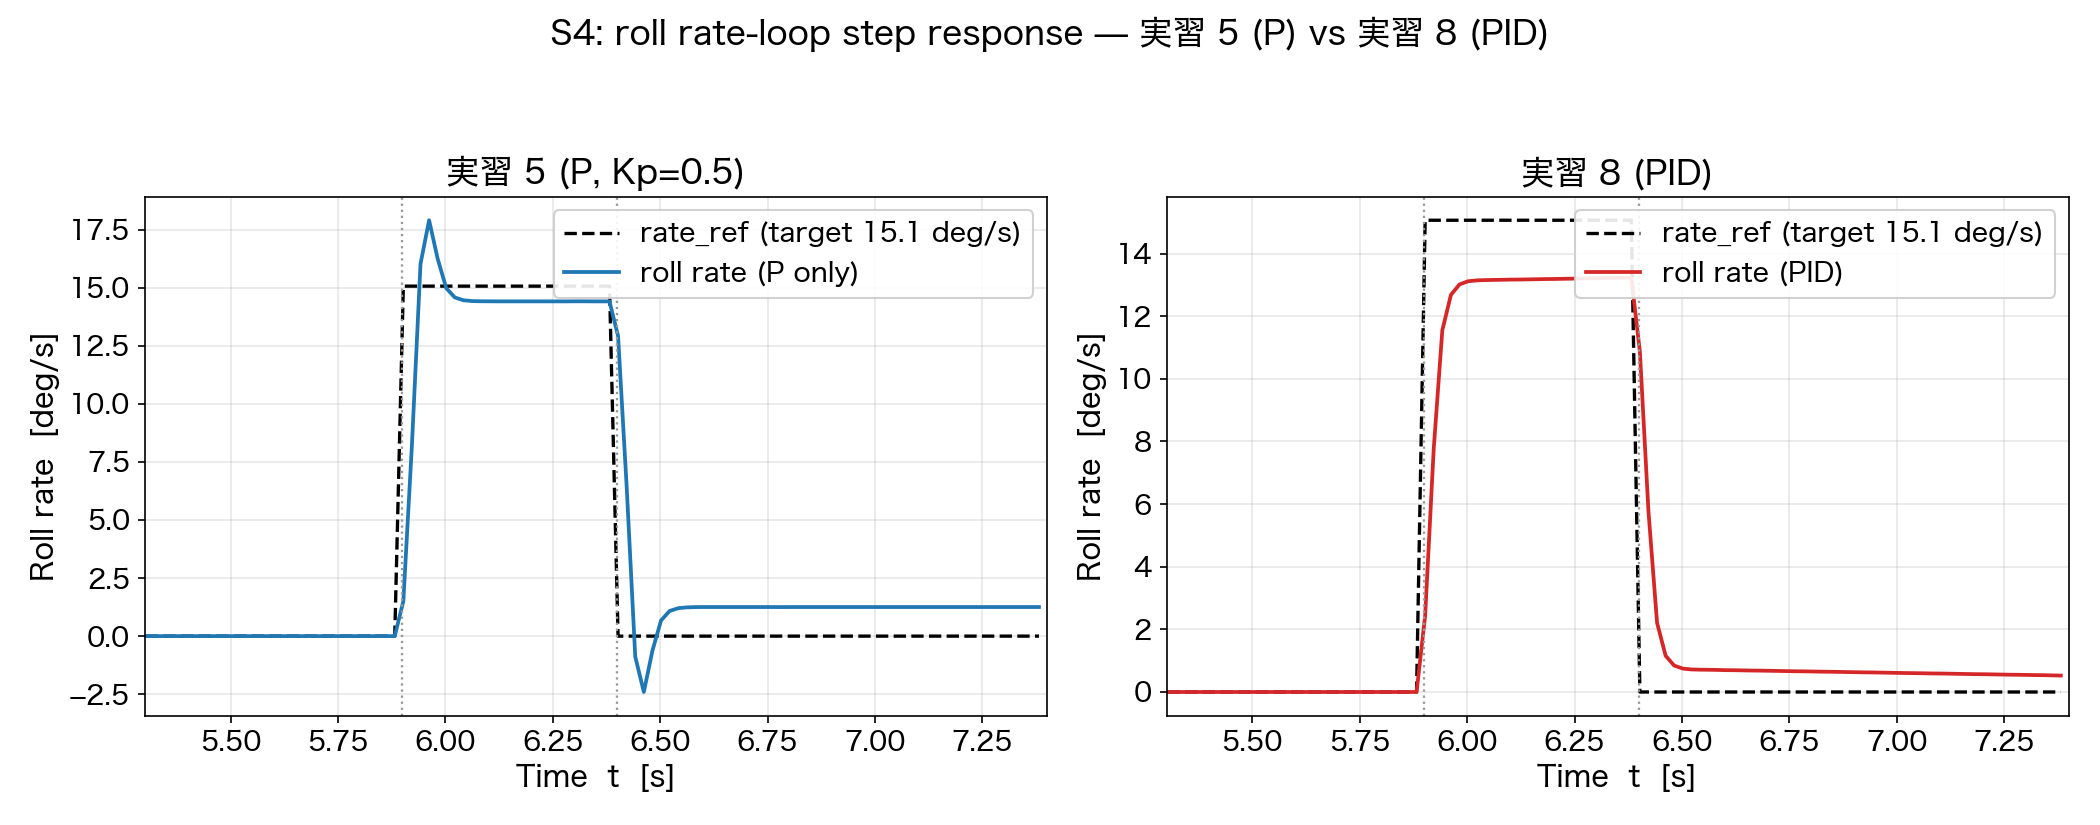
\includegraphics[width=0.94\textwidth, height=0.44\paperheight, keepaspectratio]{../fallback/S4_roll_step_p_vs_pid.png}
  \end{center}
  \vspace{-0.3em}
  \begin{itemize}\footnotesize\setlength{\itemsep}{0pt}
    \item 実習 5（P）: 目標 15.1\,deg/s に対しピーク 17.9\,deg/s の行き過ぎ。指令を戻すと $-2.4$\,deg/s まで振れ、$+1.3$\,deg/s が残る
    \item 実習 8（PID）: 行き過ぎや振動がなく、立ち上がりはゆるやか
  \end{itemize}
  {\scriptsize SILS（MuJoCo）、ロール指令 $+0.3$ を 0.5\,s。再現: \code{sf lesson switch sci2026:8 --solution}、\code{sf lesson sils --scenario step}\par}
\end{frame}


\scistep{6}{姿勢推定 --- ジャイロと加速度を混ぜる}{Step 6: 姿勢推定}
% ==============================================================================
% core_step6_attitude.tex — SCI/SICE tutorial core deck, Step 6: attitude
% estimation (exercise 9). Code values from lesson_09_estimation/solution.cpp.
% SCI/SICE チュートリアル要点版 Step 6: 姿勢推定（実習 9）。
% ==============================================================================

% ------------------------------------------------------------------
\begin{frame}{ジャイロだけでは姿勢角が求まらない}
  \begin{columns}[c]
    \begin{column}{0.48\textwidth}
      \centering
      \adjustbox{max width=\columnwidth, max height=0.66\textheight}{\documentclass[border=10pt]{standalone}
\usepackage{tikz}
\usetikzlibrary{arrows.meta}

\begin{document}

\definecolor{truecolor}{RGB}{0, 120, 200}     % Blue - true value
\definecolor{driftcolor}{RGB}{220, 50, 30}     % Red - gyro integrated
\definecolor{gridcolor}{RGB}{210, 210, 210}
\definecolor{labelcolor}{RGB}{80, 80, 80}
\definecolor{annocolor}{RGB}{40, 160, 40}      % Green - annotations

\begin{tikzpicture}[
    axis/.style={-{Stealth[length=3mm]}, line width=1pt, labelcolor},
    trueline/.style={truecolor, line width=2.5pt},
    driftline/.style={driftcolor, line width=2pt},
    dim/.style={{Stealth[length=2.5mm]}-{Stealth[length=2.5mm]}, annocolor,
                line width=1pt},
    annolbl/.style={font=\normalsize\bfseries, annocolor},
  ]

  % Grid
  \foreach \x in {0, 1, ..., 8} {
    \draw[gridcolor] (\x, 0) -- (\x, 5);
  }
  \foreach \y in {0, 1, ..., 5} {
    \draw[gridcolor] (0, \y) -- (8, \y);
  }

  % Axes
  \draw[axis] (-0.3, 0) -- (8.8, 0) node[right, font=\large\bfseries] {$t$};
  \draw[axis] (0, -0.3) -- (0, 5.5) node[above, font=\large\bfseries] {$\theta$};

  % Time labels
  \foreach \x/\t in {0/0, 2/10, 4/20, 6/30, 8/40} {
    \node[font=\small, below, labelcolor] at (\x, -0.15) {\t s};
  }

  % True value (horizontal line at y=2)
  \draw[trueline] (0, 2) -- (8, 2);
  \node[font=\normalsize\bfseries, truecolor, below] at (3, 1.85) {True angle};

  % Gyro integrated value (drifting upward)
  \draw[driftline] plot[smooth, tension=0.5] coordinates {
    (0, 2.0) (0.5, 2.05) (1, 2.15) (1.5, 2.25) (2, 2.4)
    (2.5, 2.55) (3, 2.7) (3.5, 2.85) (4, 3.05)
    (4.5, 3.2) (5, 3.4) (5.5, 3.55) (6, 3.75)
    (6.5, 3.9) (7, 4.1) (7.5, 4.25) (8, 4.45)
  };
  \node[font=\normalsize\bfseries, driftcolor, above left] at (7, 4.3)
    {Gyro $\displaystyle\int\!\omega\,dt$};

  % Drift annotation at t=40s (x=8)
  \draw[annocolor, line width=0.8pt, dashed] (8, 2.0) -- (8, 4.45);
  \draw[dim] (8.4, 2.0) -- (8.4, 4.45);
  \node[annolbl, right] at (8.5, 3.2) {Drift};

\end{tikzpicture}
\end{document}
}
    \end{column}
    \begin{column}{0.50\textwidth}
      \footnotesize
      \begin{itemize}\setlength{\itemsep}{3pt}
        \item ジャイロは角速度 $\omega$ を測る。角度は積分 $\theta=\int\omega\,dt$ で求める
        \item 測定のバイアス（偏り）も積分されるので、時間とともに誤差が増える（ドリフト）
        \item 姿勢角そのものを目標にする制御（STABILIZE 以上）には、角度の推定が要る
      \end{itemize}
      \begin{alertblock}{そこで}
        \scriptsize 重力の向きを測る加速度計で角度を補う。加速度計は長期で安定だが、短期は振動や加減速でノイズが乗る
      \end{alertblock}
    \end{column}
  \end{columns}
\end{frame}

% ------------------------------------------------------------------
\begin{frame}{相補フィルタ: ジャイロと加速度計を混ぜる}
  \begin{columns}[c]
    \begin{column}{0.48\textwidth}
      \centering
      \adjustbox{max width=\columnwidth, max height=0.62\textheight}{\documentclass[border=10pt]{standalone}
\usepackage{tikz}
\usetikzlibrary{arrows.meta, positioning, calc}

\begin{document}

\definecolor{sfblue}{RGB}{0, 120, 200}
\definecolor{sfred}{RGB}{220, 50, 30}
\definecolor{sfgreen}{RGB}{40, 160, 40}
\definecolor{sfgray}{RGB}{80, 80, 80}
\definecolor{sflight}{RGB}{220, 240, 255}

\begin{tikzpicture}[
    node distance=1.5cm and 1.5cm,
    block/.style={draw, #1, line width=1.2pt, fill=#1!8,
                  minimum width=2.0cm, minimum height=0.9cm,
                  font=\normalsize\bfseries, rounded corners=3pt},
    block/.default=sfblue,
    gain/.style={draw, #1, line width=1.2pt, fill=#1!8,
                 circle, minimum size=0.9cm,
                 font=\normalsize\bfseries},
    gain/.default=sfblue,
    % Summing-junction circle diameter ~40% of block height (Block Diagram
    % Style convention; matches feedback_block.tex / pid_block.tex).
    % 加え合わせ点の円の直径はブロック高さの約4割（ブロック線図の流儀。
    % feedback_block.tex / pid_block.tex と揃える）。
    sum/.style={draw, sfblue, line width=1.2pt, fill=white,
                circle, minimum size=0.4cm,
                font=\normalsize\bfseries},
    input/.style={font=\normalsize\bfseries, sfgray},
    output/.style={font=\large\bfseries, sfblue},
    line/.style={-{Stealth[length=2.5mm]}, line width=1.2pt, sfgray},
    pathlbl/.style={font=\normalsize\bfseries},
  ]

  % --- Main path (gyro row): omega -> x(Delta t) -> Sigma1 -> alpha -> Sigma2 -> output ---
  % 主経路（ジャイロ行）: ω → ×Δt → Σ1 → α → Σ2 → 出力
  \node[input] (gyro_in) {Gyro $\omega$};
  \node[block=sfred, right=1.3cm of gyro_in] (dt_block) {$\times\Delta t$};
  \node[sum, right=1.3cm of dt_block] (sum1) {$\Sigma$};
  \node[gain=sfred, right=1.3cm of sum1] (alpha) {$\alpha$};
  \node[sum, right=1.3cm of alpha] (sum2) {$\Sigma$};
  \node[output, right=1.1cm of sum2] (output) {$\hat{\theta}$};

  % --- Accel path (top row): drops into Sigma2 from above, entirely outside
  %     the gyro feedback loop below (which stays self-contained around
  %     Sigma1). This is the layout fix versus the previous revision, where
  %     the accel row sat below the main row and visually nested inside the
  %     feedback loop even though it carries no feedback signal. ---
  % 加速度経路（上段）: Σ2 に上から入る。下側のジャイロ・フィードバック
  % ループ（Σ1周りで閉じる）とは完全に別の場所を通る。旧版は加速度経路が
  % 主経路の下段にあり，フィードバック信号ではないのに見た目上ループの
  % 内側に入り込んでいた。これを是正したのが今回のレイアウト。
  \node[input, above=2.0cm of gyro_in] (accel_in) {Accel};
  \node[block=sfgreen, right=1.3cm of accel_in] (atan) {atan2};
  \node[gain=sfgreen, right=1.3cm of atan] (one_alpha) {$1\!-\!\alpha$};

  % --- Feedback delay path (below row): previous estimate theta_hat_{k-1} ---
  % フィードバック遅延経路（下段）: 前回推定値 θ̂_{k-1} を戻す
  \node[block=sfblue, below=1.5cm of sum1, minimum width=1.6cm] (delay) {$z^{-1}$};

  % --- Branch point on the output line (theta_hat is tapped, not re-derived) ---
  % 出力線上の分岐点（θ̂ をそのまま分岐、再計算しない）
  \coordinate (tap) at ($(sum2)!0.5!(output)$);

  % --- Connections: gyro path ---
  \draw[line, sfred] (gyro_in) -- (dt_block);
  \draw[line, sfred] (dt_block) -- (sum1.west);
  \draw[line, sfred] (sum1.east) -- (alpha.west);
  \draw[line, sfred] (alpha.east) -- (sum2.west);

  % --- Connections: accel path. Drops straight down into Sigma2 from the
  %     north; a short right-angle jog (down, then across) absorbs the
  %     small misalignment between one_alpha's x-position and sum2's,
  %     since "right=1.3cm of" spacing is computed from each row's own
  %     node widths and the two rows use different-width nodes. ---
  % 加速度経路の接続。Σ2 に北側からまっすぐ下りる。one_alpha と sum2 の
  % x座標のわずかなズレ（"right=1.3cm of" の間隔は各行のノード幅から
  % 計算されるため，幅の違う行同士では厳密には揃わない）を、
  % 短い直角ジョグ（下りてから横に寄せる）で吸収する。
  \draw[line, sfgreen] (accel_in) -- (atan);
  \draw[line, sfgreen] (atan) -- (one_alpha);
  \draw[line, sfgreen] (one_alpha.south) -- ++(0,-0.4) -| (sum2.north);

  % --- Output line and its branch dot ---
  \draw[line, sfblue, line width=1.5pt] (sum2) -- (output);
  \fill[sfblue] (tap) circle (2.2pt);

  % --- Feedback path: branch dot -> straight down -> into delay from the
  %     east -> up into Sigma1 from below. With the accel path now routed
  %     above the main row, the lower half-plane belongs to this path
  %     alone, so (unlike the previous revision) no detour around another
  %     signal is needed. ---
  % フィードバック経路: 分岐点 → まっすぐ下へ → 遅延ブロックへ東側から
  % 入る → 上へ → Σ1 に南側から入る。加速度経路が上段に移ったことで
  % 下半分はこの経路専用になり，旧版で必要だった他信号を避ける迂回が
  % 不要になった。
  \draw[line, sfblue] (tap) -- (tap |- delay.east) -- (delay.east);
  \draw[line, sfblue] (delay.north) -- (sum1.south);

  % --- Sum node signs (Block Diagram Style convention): "+" sits above a
  %     horizontally (west-)entering arrow. For a vertically-entering arrow
  %     (into Sigma1 from below, into Sigma2 from above) the "+" sits to
  %     the arrow's right, mirroring Sigma1's existing bottom-entry sign. ---
  % 加え合わせ点の符号（ブロック線図の流儀）: 水平（西側）から入る矢印の
  % 「＋」はその上に置く。垂直に入る矢印（Σ1は下から，Σ2は上から）の
  % 「＋」はその右側に置く（Σ1の下からの入力の符号と同じ規則）。
  \node[font=\scriptsize, sfred,  anchor=south east] at ($(sum1.north)+(150:0.3)$) {$+$};
  \node[font=\scriptsize, sfblue, anchor=north west] at ($(sum1.south)+(330:0.3)$) {$+$};
  \node[font=\scriptsize, sfred,  anchor=south east] at ($(sum2.north)+(150:0.3)$) {$+$};
  \node[font=\scriptsize, sfgreen, anchor=south west] at ($(sum2.north)+(30:0.3)$) {$+$};

  % --- Path labels (kept off the signal lines) ---
  \node[pathlbl, sfred, below=0.2cm of dt_block] {High-pass};
  \node[pathlbl, sfgreen, above=0.2cm of atan] {Low-pass};
  \node[pathlbl, sfblue, below=0.15cm of delay] {前回値};

\end{tikzpicture}
\end{document}
}
    \end{column}
    \begin{column}{0.50\textwidth}
      \footnotesize
      \setlength{\abovedisplayskip}{2pt}\setlength{\belowdisplayskip}{2pt}%
      静止時の加速度計は重力の反力を測るので、傾きが求まる（$\phi$: ロール、$\theta$: ピッチ）:
      \[
        \begin{aligned}
        \phi_a&=\operatorname{atan2}(-a_y,-a_z)\\
        \theta_a&=\operatorname{atan2}\bigl(a_x,\sqrt{a_y^2+a_z^2}\bigr)
        \end{aligned}
      \]
      相補フィルタ（$\alpha=0.98$）:
      \[
        \hat\theta_k=\alpha(\hat\theta_{k-1}+\omega\,\Delta t)+(1-\alpha)\theta_a
      \]
      短期はジャイロ、長期は加速度計を使う（互いの弱点を補う）。ヨー角は重力から求まらない
    \end{column}
  \end{columns}
\end{frame}

% ------------------------------------------------------------------
\begin{frame}[fragile]{実習 9: 相補フィルタを実装し、機体の推定と比べる}
  \exgoal{自作の相補フィルタの角度を、機体既定の推定器 ESKF（誤差状態カルマンフィルタ）と比べる}
  \begin{columns}[T]
    \begin{column}{0.46\textwidth}
      {\footnotesize\textbf{\textcolor{sfblue}{手順（飛行しない）}}}\par\vspace{-2pt}
        \footnotesize
        \begin{enumerate}\setlength{\itemsep}{0pt}
          \item \code{sf lesson switch sci2026:9}
          \item \code{sf lesson edit} で右のコードにして保存
          \item \code{sf lesson build}、\code{sf lesson flash}
          \item \code{sf lesson monitor}、Teleplot で \code{cf\_roll} と \code{eskf\_roll} を重ねる
        \end{enumerate}
    \end{column}
    \begin{column}{0.52\textwidth}
      \begin{sflisting}[basicstyle=\ttfamily\scriptsize, moredelim={[is][\bfseries\color{sfred}]{<<}{>>}}]{user\_code.cpp（赤字を書く）}
<<float a_roll = atan2f(-ay, -az);>>
<<float a_pitch = atan2f(ax,>>
<<    sqrtf(ay*ay + az*az));>>
<<cf_roll = alpha*(cf_roll + gx*dt)>>
<<         + (1-alpha)*a_roll;>>
// pitch: same form (gy, a_pitch)
<<ws::print(">cf_roll:%.2f", ...);>>
<<ws::print(">eskf_roll:%.2f", ...);>>
      \end{sflisting}
    \end{column}
  \end{columns}
  \exresult{機体を手で傾けると 2 つの角度がほぼ一致して動く。$\alpha$ を変えて違いを見る}
  \exhelptodo{9}
\end{frame}


% === まとめ ===
\gdef\sciFooterSession{まとめ}
% ==============================================================================
% core_summary.tex — SCI/SICE tutorial core deck: summary
% SCI/SICE チュートリアル要点版: まとめ
% ==============================================================================

% ------------------------------------------------------------------
\begin{frame}{今日やったこと}
  \begin{table}
    \centering\footnotesize
    \begin{tabular}{llp{62mm}}
      \hline
      \textbf{Step} & \textbf{実習} & \textbf{得たもの} \\
      \hline
      1 センサ & 2 & 軸と符号、IMU の値の見方 \\
      2 モータとミキサ & 3, 4 & Duty、ミキサ、開ループでは飛べない理由 \\
      3 P 制御とモデル & 5, 6 & $G_p=K/(s(\tau_m s+1))$、$K_p=1/(4\zeta^2K\tau_m)$ \\
      4 システム同定 & 7 & 飛行データから $K,\tau_m$ を推定し、理論値と照合 \\
      5 PID & 8 & I 項・D 項の役割、SILS での確認 \\
      6 姿勢推定 & 9 & 相補フィルタ（ジャイロ + 加速度計） \\
      \hline
    \end{tabular}
  \end{table}
  \vspace{0.2em}
  {\footnotesize 設計 $\to$ 実装 $\to$ 実験 $\to$ 解析を、1 機で一周した\par}
\end{frame}

% ------------------------------------------------------------------
\begin{frame}{この先へ}
  \begin{table}
    \centering\footnotesize
    \begin{tabular}{>{\raggedright\arraybackslash}p{40mm}>{\raggedright\arraybackslash}p{80mm}}
      \hline
      \textbf{したいこと} & \textbf{入口} \\
      \hline
      自分の制御器・推定器を載せる & \code{sf app new <名前>}。入門は \code{docs/guides/custom\_program.md} \\
      シミュレータをブラウザで触る & \code{sf sils build}、\code{sf sils gui} \\
      位相余裕・むだ時間、不完全微分、周波数同定、自動チューニングなど & 現行版スライド \code{slides/sci\_tutorial.pdf} の第 4・5 セッション \\
      復習の手順・コマンド・API の早見表 & \code{handson\_guide.md}、\code{cheatsheet.md}（同じフォルダ） \\
      \hline
    \end{tabular}
  \end{table}
  {\scriptsize リポジトリ: \url{https://github.com/M5Fly-kanazawa/stampfly_ecosystem} ／ 資料: \url{https://www.docswell.com/s/Kouhei_Ito/5L387D-2026-09-10-064635}\par}
\end{frame}

% ------------------------------------------------------------------
\begin{frame}[fragile]{コマンド早見表}
  \begin{table}
    \centering\footnotesize
    \begin{tabular}{>{\raggedright\arraybackslash}p{74mm}>{\raggedright\arraybackslash}p{54mm}}
      \hline
      \code{sf doctor} & 環境診断（困ったらまずこれ） \\
      \code{sf lesson switch sci2026:N [--solution]} & 実習 N の雛形（解答）に切り替え \\
      \code{sf lesson edit / build / flash / monitor} & 編集・ビルド・書き込み・モニタ \\
      \code{sf lesson sils [--scenario step]} & 実習コードを SILS で確認 \\
      \code{sf telemetry} & 50\,Hz の状態をライブ表示（WiFi） \\
      \code{sf log wifi -d 30} & 400\,Hz で記録（WiFi） \\
      \code{sf log list} / \code{sf log viz} & ログ一覧 / 最新ログの可視化 \\
      \code{sf sysid fit <ログ> --plot} & プラント同定 \\
      \hline
    \end{tabular}
  \end{table}
\end{frame}

% ------------------------------------------------------------------
\begin{frame}{困ったとき}
  \begin{table}
    \centering\footnotesize
    \begin{tabular}{>{\raggedright\arraybackslash}p{38mm}>{\raggedright\arraybackslash}p{82mm}}
      \hline
      \textbf{症状} & \textbf{対処} \\
      \hline
      ビルドエラー & エラー 1 行目のファイル名・行番号を見て、コードの打ち間違い（カンマ、セミコロン）を直す \\
      \code{sf lesson flash} が失敗 & 別のケーブル・ポートを試す。だめなら機体の BOOT ボタン（基板上の、書き込み専用モードに入るボタン）を押したまま USB を挿し直す \\
      モータが回らない & ARM されていない。USB 給電中・ペアリング中は ARM が拒否されるので、USB を外し、水平な机に置く。ALT/POS モードでは自動離陸に入るので OFF にする \\
      LED が緑にならない & 起動時の校正中に動かした。静かに置き直し、緑とビープ 3 回を待つ \\
      機体の WiFi が見えない & 電源と \code{wifi.mode 1} を確認 \\
      \code{sf doctor} が通らない & 表示された項目を確認し、\code{docs/guides/troubleshooting.md} を見る \\
      \hline
    \end{tabular}
  \end{table}
\end{frame}


\end{document}
